%============================================================= 
% Identity After Collapse 
% Self-Reference and Normal-Form Fixed Points 
% A Theory of Trace and Evaluation in Irreversible Systems %============================================================= 


\documentclass[12pt, oneside]{amsbook}

%-------------------------------------------------------------
% PACKAGES
%-------------------------------------------------------------
\usepackage{geometry}
\geometry{
  paper=a4paper,
  top=30mm, bottom=30mm,
  inner=30mm, outer=28mm,
  marginparwidth=0mm,
  marginparsep=0mm
}

\usepackage[T1]{fontenc}
\usepackage[utf8]{inputenc}
% microtype disabled (font expansion unavailable in this environment)

% Math
\usepackage{amsmath, amssymb, amsthm}
\usepackage{mathtools}
\usepackage{stmaryrd}
\usepackage{bm}

% Graphics and colour
\usepackage{xcolor}
\usepackage{tikz}
\usetikzlibrary{arrows.meta, positioning, calc, shadings, fadings, perspective, 3d}
\usepackage{tikz-cd}

% Boxes
\usepackage{tcolorbox}
\tcbuselibrary{theorems, breakable, skins}

% Layout
\usepackage{setspace}
\usepackage{titlesec}
\usepackage{parskip}
\usepackage{fancyhdr}
\usepackage{enumitem}
\usepackage{booktabs}
\usepackage{array}

% References
\usepackage[numbers, sort&compress]{natbib}
\usepackage{hyperref}
\usepackage{cleveref}
\usepackage{url}
\usepackage{csquotes}

%-------------------------------------------------------------
% COLOURS
%-------------------------------------------------------------
\definecolor{spblue}{RGB}{25, 60, 100}
\definecolor{sprust}{RGB}{139, 58, 30}
\definecolor{spgold}{RGB}{160, 120, 30}
\definecolor{spgray}{RGB}{100, 96, 88}
\definecolor{splightgray}{RGB}{240, 237, 230}
\definecolor{spsage}{RGB}{60, 95, 70}

%-------------------------------------------------------------
% HYPERREF
%-------------------------------------------------------------
\hypersetup{
  colorlinks = true,
  linkcolor  = spblue,
  citecolor  = sprust,
  urlcolor   = spsage,
  pdftitle   = {Identity After Collapse},
  pdfauthor  = {Flyxion},
}

%-------------------------------------------------------------
% THEOREM ENVIRONMENTS
%-------------------------------------------------------------
\theoremstyle{plain}
\newtheorem{theorem}{Theorem}[section]
\newtheorem{proposition}[theorem]{Proposition}
\newtheorem{lemma}[theorem]{Lemma}
\newtheorem{corollary}[theorem]{Corollary}
\newtheorem{conjecture}[theorem]{Conjecture}

\theoremstyle{definition}
\newtheorem{definition}[theorem]{Definition}
\newtheorem{example}[theorem]{Example}
\newtheorem{construction}[theorem]{Construction}
\newtheorem{notation}[theorem]{Notation}
\newtheorem{assumption}[theorem]{Assumption}

\theoremstyle{remark}
\newtheorem{remark}[theorem]{Remark}

%-------------------------------------------------------------
% TCOLORBOX STYLES
%-------------------------------------------------------------
\tcbset{
  spbox/.style={
    enhanced, breakable,
    colback=splightgray, colframe=spgray,
    arc=2pt, boxrule=0.5pt,
    left=7pt, right=7pt, top=5pt, bottom=5pt,
    fonttitle=\small\bfseries\sffamily,
  },
  hinge/.style={
    spbox,
    colframe=sprust, colback=sprust!5!white,
    borderline west={2.5pt}{0pt}{sprust},
  },
  priest/.style={
    spbox,
    colframe=spgold, colback=spgold!5!white,
    borderline west={2.5pt}{0pt}{spgold},
  },
  reduction/.style={
    enhanced, breakable,
    colback=spblue!4!white, colframe=spblue!30!white,
    arc=2pt, boxrule=0.5pt,
    left=9pt, right=7pt, top=5pt, bottom=5pt,
    fontupper=\small\ttfamily,
  },
}

%-------------------------------------------------------------
% OPERATORS & MACROS
%-------------------------------------------------------------
\newcommand{\Expr}{\mathcal{E}}
\newcommand{\NF}{\mathcal{N}}
\newcommand{\Traj}{\mathcal{T}}
\newcommand{\evalf}{f}
\newcommand{\trace}{\tau}
\newcommand{\collapseop}{\mathsf{collapse}}
\newcommand{\bind}{\mathsf{bind}}
\newcommand{\pop}{\mathsf{pop}}
\newcommand{\refuse}{\mathsf{refuse}}
\newcommand{\nf}[1]{\operatorname{nf}(#1)}
\newcommand{\tequiv}{\sim}
\newcommand{\preimgset}[1]{f^{-1}(#1)}
\newcommand{\ruleR}{\mathcal{R}}
\newcommand{\eventword}{\partial}

\newcommand{\docens}{\textit{logica~docens}}
\newcommand{\utens}{\textit{logica~utens}}
\newcommand{\ens}{\textit{logica~ens}}
\newcommand{\Docens}{\textit{Logica~Docens}}
\newcommand{\Utens}{\textit{Logica~Utens}}
\newcommand{\Ens}{\textit{Logica~Ens}}

\newcommand{\CStr}{\mathrm{CStr}}
\newcommand{\FStr}{\mathrm{FStr}}
\newcommand{\HLFGproj}{\Pi_{\mathrm{func}}}

\newcommand{\feat}[1]{\left[\begin{array}{ll}#1\end{array}\right]}

\newcommand{\RSVPfield}{\Phi}
\newcommand{\RSVPvec}{\mathbf{v}}
\newcommand{\entropyF}{\mathcal{F}}

%-------------------------------------------------------------
% PAGE STYLE
%-------------------------------------------------------------
\pagestyle{fancy}
\fancyhf{}
\fancyhead[L]{\small\textcolor{spgray}{\textit{Identity After Collapse}}}
\fancyhead[R]{\small\textcolor{spgray}{\nouppercase{\leftmark}}}
\fancyfoot[C]{\small\textcolor{spgray}{\thepage}}
\renewcommand{\headrulewidth}{0.3pt}
\renewcommand{\headrule}{%
  \hbox to\headwidth{\color{spgray!60}\leaders\hrule height\headrulewidth\hfill}}

%-------------------------------------------------------------
% SECTION FORMATTING
%-------------------------------------------------------------
\titleformat{\chapter}[display]
  {\normalfont\Large\bfseries\color{spblue}}
  {\chaptertitlename\ \thechapter}{12pt}{\huge}
  [\vspace{4pt}\textcolor{spgray!50}{\rule{\linewidth}{0.4pt}}]

\titleformat{\section}
  {\normalfont\large\bfseries\color{spblue}}
  {\thesection}{1em}{}

\titleformat{\subsection}
  {\normalfont\normalsize\bfseries\color{spgray}}
  {\thesubsection}{1em}{}

%-------------------------------------------------------------
% SPACING
%-------------------------------------------------------------
\setstretch{1.18}
\setlength{\parindent}{0pt}
\setlength{\parskip}{6pt plus 2pt minus 1pt}

%=============================================================
\begin{document}

% ── TOC and numbering settings ──
\setcounter{secnumdepth}{0}   % chapters numbered; sections/subsections not
\setcounter{tocdepth}{2}       % TOC shows chapters and sections

%=============================================================

%-------------------------------------------------------------
% TITLE PAGE
%-------------------------------------------------------------
\begin{titlepage}
  \centering
  \vspace*{2cm}
  {\Large\textcolor{spgray}{\textsc{Monograph in Formal Computation and Philosophy of Logic}}}
  \\[1.8cm]
  {\Huge\bfseries\color{spblue} Identity After Collapse}\\[0.6cm]
{\Large\itshape Self-Reference and Normal-Form Fixed Points}\\[0.5cm]
{\normalsize\textcolor{spgray}{A Theory of Trace and Evaluation in Irreversible Systems}}\\[2.5cm]
\textcolor{spgray!60}{\rule{9cm}{0.4pt}}\\[1.2cm]
{\large Flyxion}\\[0.4cm]
  {\normalsize\textcolor{spgray}{Independent Researcher}}\\[2cm]
  {\normalsize\textcolor{spgray}{\today}}
  \vfill
\end{titlepage}

%-------------------------------------------------------------
% ABSTRACT
%-------------------------------------------------------------
\cleardoublepage
\chapter*{Abstract}

We develop a formal theory of self-reference for calculi governed by
\emph{irreversible reduction}. The evaluation map of the Spherepop calculus
is a one-way collapse of nested structure into a terminal trace, and this map
has no right inverse. Classical quines---programs that reproduce their own
source---are therefore impossible: the preimage is destroyed and cannot be
recovered. In their place we introduce \emph{normal-form fixed points},
expressions whose identity survives as an invariant of their own collapse.

We show that irreversibility forces a divergence in Graham Priest's tripartite
distinction between logica docens, utens, and ens, relocating validity from
syntactic preservation to trace stability. The framework extends to natural
language via Historical Lexical-Functional Grammar, where grammatical structure
is the residue of irreversible constraint elimination. It extends further to
asynchronous circuit logic, categorical sheaf theory, and RSVP field dynamics,
where identity corresponds to entropic attractors. Spherepop is shown to be
computationally equivalent to the lambda calculus and hence to Turing machines,
grounding these contributions in the standard theory of computation.

At fixed points, program, execution, and description collapse into one object.
A Spherepop quine does not reproduce itself; it \emph{is} its own result.

\medskip\noindent
\textbf{Keywords:}\ irreversible reduction, Spherepop, trace identity,
normal-form fixed points, quines, logica ens, lambda calculus,
Turing completeness, Historical LFG, sheaf of histories, RSVP.

%-------------------------------------------------------------
% TABLE OF CONTENTS
%-------------------------------------------------------------
\tableofcontents

%=============================================================
\part{Grounding: Making Evaluation Visible}
%=============================================================

%-------------------------------------------------------------
\chapter{Introduction: From Evaluation to Irreversibility}
\label{ch:intro}
%-------------------------------------------------------------

Standard accounts of computation present evaluation as a function: an
expression is given, a value is returned, and the process connecting the two
is treated as incidental. Whether in arithmetic, lambda calculus, or programming
languages, the dominant formal picture suppresses the internal structure of
evaluation in favour of its input--output behaviour. This suppression is not
merely a matter of convenience. It reflects a deeper assumption: that the
process of evaluation is, in principle, reversible or at least reconstructible
from its result.

The aim of this work is to examine what happens when this assumption is removed.

We begin from a simple observation. In many concrete systems, evaluation does
not preserve the information required to reconstruct its starting point. When
an arithmetic expression such as
\[
  (8 + (3 \times 5))
\]
is reduced to the value $23$, the intermediate structure that justified this
result is no longer present. The result does not encode its own derivation.
Distinct expressions may collapse to the same value, and no operation defined
purely on the value can recover which expression produced it. Evaluation, in
such cases, is not a reversible transformation but a \emph{collapse}.

This observation motivates a shift in perspective. Rather than treating
evaluation as a mapping between static objects, we treat it as a sequence of
irreversible events. Each step in a reduction trajectory eliminates
possibilities, contracts structure, and commits the system to a narrower range
of future states. What survives this process is not the history itself, but a
terminal invariant: the \emph{trace}.

\begin{tcolorbox}[hinge]
  \textbf{Central Question.}\ What is identity in a system where evaluation
  irreversibly destroys its own preimage?
\end{tcolorbox}

In reversible settings, identity may be defined syntactically or
extensionally: an expression is identical to itself if its structure is
preserved, or if it can be reconstructed from its value. Under irreversible
collapse, neither of these criteria is available. The result of evaluation does
not determine its origin, and distinct histories may converge to the same
terminal state. Identity must therefore be relocated from the domain of initial
configurations to the domain of what persists after collapse.

This relocation has immediate consequences for self-reference. The classical
notion of a quine---a program that produces its own source as output---depends
on the ability to preserve or encode syntactic structure across evaluation.
If evaluation destroys preimage information, such reproduction becomes
impossible. The question is not how a program can reproduce itself, but how it
can remain itself under projection onto its terminal trace.

To make this question precise, we introduce the Spherepop calculus, a minimal
formal system in which evaluation is explicitly irreversible. In Spherepop,
expressions are built from nested bubbles, and evaluation consists of popping
these bubbles according to local reduction rules. Each pop removes a layer of
structure and cannot be undone. The calculus therefore makes visible what
standard presentations conceal: evaluation as a sequence of commitments that
progressively eliminate alternative possibilities.

Within this setting, we develop a theory of identity as trace invariance. The
evaluation map $\evalf : \Expr \to \NF$ is shown to have no right inverse: the
preimage of a normal form is not recoverable. This forces a redefinition of
identity in terms of equivalence under collapse. Two expressions are identical
not because they share a derivation, but because they share a trace.

This shift is further clarified through the integration of Graham Priest's
distinction between \docens{}, \utens{}, and \ens{}. In reversible systems,
these strata are often implicitly conflated. In an irreversible calculus, they
diverge. The formal rules of reduction, the practice of evaluation, and the
resulting facts of validity become distinct objects, connected only through the
process of collapse. Identity emerges at the level of \ens{}: the invariant
trace that survives all trajectories.

The consequences extend beyond abstract computation. By reinterpreting lexical
events as irreversible operations over a grammatical option space, we derive
a Historical Lexical-Functional Grammar in which syntactic and functional
structure are not independent representations but the residue of a shared
process of constraint elimination. Grammaticality becomes the existence of a
non-empty terminal trace; ungrammaticality becomes total collapse.

At the limit of this development lies a new notion of self-reference. A
Spherepop quine is not an expression that reproduces its own source, but one
whose evaluation yields a trace equivalent to itself. At such fixed points,
the distinction between program, execution, and description disappears. The
expression is identical with the result of its own collapse.

The argument proceeds in stages. Part~I (Chapters~\ref{ch:visible}
and~\ref{ch:spherepop}) makes evaluation visible as a sequence of reduction
events and introduces the Spherepop calculus as a formal system of irreversible
commitment. Part~II (Chapter~\ref{ch:collapse}) establishes the central
structural fact: the evaluation map has no right inverse. This asymmetry is the
hinge on which the entire theory turns. Chapter~\ref{ch:identity} develops
identity as equivalence under trace, and Chapter~\ref{ch:priest} situates the
framework within Priest's tripartite logical stratification. Part~III
(Chapters~\ref{ch:fixedpoints} and~\ref{ch:pec}) reconstructs self-reference
in this setting. Classical quines are shown to fail; in their place we introduce
normal-form fixed points and the Spherepop quine. At these points the distinction
between representation and meaning collapses. Part~IV
(Chapters~\ref{ch:hlfg} and~\ref{ch:parse}) extends the framework to natural
language, deriving a Historical Lexical-Functional Grammar and demonstrating its
operation through a worked parse. Chapter~\ref{ch:empirical} outlines empirical
consequences, and Chapter~\ref{ch:conclusion} states the general result.

The guiding intuition throughout is simple but far-reaching. Evaluation is not
a reversible transformation of form, but a process of elimination. Possibilities
are progressively excluded until only a stable configuration remains. That
configuration does not represent its origin; it is what remains after the
origin has been irreversibly transformed. To understand identity in such a
system is therefore to understand what survives collapse.

%-------------------------------------------------------------
\chapter{Making Evaluation Visible}
\label{ch:visible}
%-------------------------------------------------------------

Standard presentations of computation describe evaluation as a mapping from
expressions to values. This description suppresses the internal structure of
evaluation, treating the process as a black box whose only relevant property is
its input--output behaviour. In this chapter, that abstraction is suspended and
evaluation is made explicit as a sequence of local transformations.

The purpose is not to introduce a new formalism, but to expose a feature
already present in ordinary computation: evaluation proceeds by the progressive
elimination of structure. Each step removes a portion of the expression and
replaces it with a value. Once removed, that structure is not retained by the
result. Evaluation is therefore not merely the computation of a value, but a
process of irreversible simplification.

\paragraph{Analogy.}
Consider peeling and chopping an onion. The act of chopping commits the onion to a particular configuration from which it cannot be restored. One cannot recover the original intact onion from the pile of chopped pieces, even though the chopped pieces represent the ``output'' of the operation. Evaluation in the Spherepop calculus works in exactly this way. The nested bubble $(3 \times 5)$ is the intact onion; the result $15$ is what remains after the structural integrity of the subexpression has been committed. The scaffolding---the fact that it was a multiplication of $3$ and $5$---is gone.

\section{Prerequisites}

This chapter assumes no formal background beyond elementary arithmetic and a passing familiarity with the idea of a computer program. The purpose is to destabilise a picture that most readers already hold implicitly, so prior technical knowledge is not required and may even be an obstacle. Readers who have worked with rewriting systems or formal language theory should read this chapter as a reframing rather than an introduction.

\section{Traces and the \texttt{pop*} Notation}
\label{sec:visible:traces}

Consider the arithmetic expression $8 + 3 \times 5$. Rather than invoking a
precedence rule, the expression may be written with its implicit structure made
explicit:
\[
  (8 + (3 \times 5)).
\]
Evaluation proceeds by reducing the innermost subexpression first. This process
is recorded as a reduction trace, in which each step explicitly displays the
current state of the expression. The notation \texttt{pop*} marks the moment at
which a subexpression is irreversibly replaced by its value.

\begin{tcolorbox}[reduction, title={Reduction trace: $8 + 3 \times 5$}]
( 8 + ( 3 * 5 ) )
( 8 + ( 15 ) )       [pop*: 3 * 5 -> 15]
( 8 + 15 )
( 23 )               [pop*: 8 + 15 -> 23]
23
\end{tcolorbox}

Two structural features are evident in this trace. Evaluation proceeds locally,
with each step acting on a single subexpression. At the same time, each
application of \texttt{pop*} removes structure. The expression $(3 \times 5)$
is replaced by $15$, and the multiplicative structure that generated this value
is no longer present. The value itself does not encode the operation or operands
from which it arose. That information has been eliminated.

\section{Left-Grouped Evaluation}
\label{sec:visible:leftgrouped}

To emphasise that this behaviour is independent of operator precedence,
consider an explicitly grouped expression:
\[
  ((12 - 4) \times 3) + 2.
\]

\begin{tcolorbox}[reduction, title={Reduction trace: $(12-4)\times 3+2$}]
( ( ( 12 - 4 ) * 3 ) + 2 )
( ( 8 * 3 ) + 2 )            [pop*: 12 - 4 -> 8]
( 24 + 2 )                   [pop*: 8 * 3 -> 24]
26                           [pop*: 24 + 2 -> 26]
\end{tcolorbox}

Here the grouping is fixed from the outset, yet the same phenomenon occurs.
Structure is introduced in order to organise evaluation and is subsequently
removed as each operation is performed. Intermediate forms exist only
transiently; they do not persist in the final result.

\section{Evaluation as Construct and Erase}
\label{sec:visible:construct-erase}

The traces above support a general characterisation of evaluation. Structural
organisation is introduced to determine how computation proceeds, but once a
subexpression has been evaluated, the structure that enabled that evaluation is
no longer required and is eliminated.

Evaluation can therefore be understood as a process in which structure is first
constructed, then utilised, and finally erased. The conventional notion of
operator precedence may be reinterpreted within this framework. Precedence does
not describe a hierarchy inherent in the final result, but rather prescribes
how a temporary hierarchy is constructed so that it may be systematically
removed. What remains at the end of evaluation is not the structured expression
but its terminal value. The scaffolding that governed the computation has been
consumed by the process itself.

\section{Irreversibility in Ordinary Computation}
\label{sec:visible:irreversibility}

The elimination of structure has an immediate and decisive consequence. The
final value does not determine the expression from which it was obtained.

In the earlier example, both $(8 + (3 \times 5))$ and $(8 + 15)$ reduce to the
same value $23$. From the value alone, it is not possible to recover which
expression was evaluated. The information distinguishing these expressions has
been irreversibly lost.

This phenomenon is not specific to arithmetic notation but arises whenever
evaluation replaces structured expressions with simpler forms. Distinct inputs
may converge to the same output, and the output does not retain the information
necessary to distinguish among them. Evaluation is therefore intrinsically
many-to-one. Irreversibility is not an exotic feature introduced by specialised
systems. It is already present in ordinary computation, though typically
concealed by the focus on final results.

\section{The Trace as Residual Structure}
\label{sec:visible:trace}

Although the internal structure of an expression is eliminated during
evaluation, the reduction trace provides a record of the process by which the
value was obtained. The trace preserves the sequence of transformations, even
as each transformation removes part of the structure.

This suggests a fundamental distinction. An expression may be identified with
its final value, in which case evaluation appears as a mapping between static
objects. Alternatively, it may be identified with the history of its reduction,
in which case evaluation is a process whose structure persists only in the
trace. Standard accounts privilege the former perspective and treat the latter
as an implementation detail. In what follows, the trace is taken to be primary,
and the final value is understood as a projection of that trace.

\section{Transition to Formalisation}
\label{sec:visible:transition}

The preceding analysis establishes that evaluation is a dynamic process
characterised by local transformation, structural elimination, and irreversible
loss of information. These features motivate the introduction of a formal
system in which irreversibility is not implicit but explicit.

In the next chapter, the Spherepop calculus is defined. Expressions are
constructed as nested structures, and evaluation proceeds through the
irreversible popping of these structures. Within that framework, the behaviour
observed here is no longer incidental. Evaluation becomes a systematic
contraction of structure, and the only invariant that survives is the terminal
trace.

%-------------------------------------------------------------
\chapter{Spherepop as an Irreversible Calculus}
\label{ch:spherepop}
%-------------------------------------------------------------

The preceding chapter established that ordinary evaluation proceeds through the
progressive elimination of structure and does not preserve the information
required to reconstruct its origin. In this chapter, that behaviour is made
explicit. We introduce the Spherepop calculus as a formal system in which
evaluation is not merely irreversible in practice, but irreversible by design.

The aim is not to replace existing rewriting systems, but to isolate and
formalise a feature they implicitly exhibit. In Spherepop, expressions are
constructed from nested structures, and evaluation consists of eliminating those
structures through local operations. Each step contracts the expression and
cannot be undone. The result is a calculus in which reduction is best understood
as a history of commitments rather than a reversible transformation.

\section{Prerequisites}

This chapter assumes familiarity with inductive definitions and elementary rewriting systems at the level of an undergraduate course in theoretical computer science or formal languages. The reader should understand what it means for a rule to be applied locally to a subexpression and should be comfortable with the distinction between an expression and its value. Familiarity with the lambda calculus is helpful but not required; the Spherepop calculus is developed from first principles. The reduction trace notation introduced in Chapter~2 is used throughout.

\section{Tokens and Bubbles}
\label{sec:sp:tokens}

\begin{definition}[Spherepop Expressions]
\label{def:sp-expr}
The set $\Expr$ of \emph{Spherepop expressions} is defined inductively. Every
atomic token $t \in \mathcal{A}$ is an expression. If $E_1, \ldots, E_n$ are
expressions, then the concatenation enclosed in parentheses
$(E_1 \cdots E_n)$ is also an expression, referred to as a \emph{bubble}.
\end{definition}

A bubble may be understood as a bounded region of structural commitment. Its
contents are grouped together so that they may be acted upon as a unit. The
nesting of bubbles therefore determines the scope within which local operations
may occur.

Unlike conventional abstract syntax trees, bubbles are not intended as a static
representation of hierarchical structure. They are transient organisational
devices whose role is to delimit the domain of reduction. Once a bubble has been
resolved, it is removed, and its internal structure does not persist in the
result.

%------------------------------------------------------------------
% FIG 3 — Spherepop Bubble Geometry (Chapter 2)
%------------------------------------------------------------------
\begin{figure}[htbp]
\centering
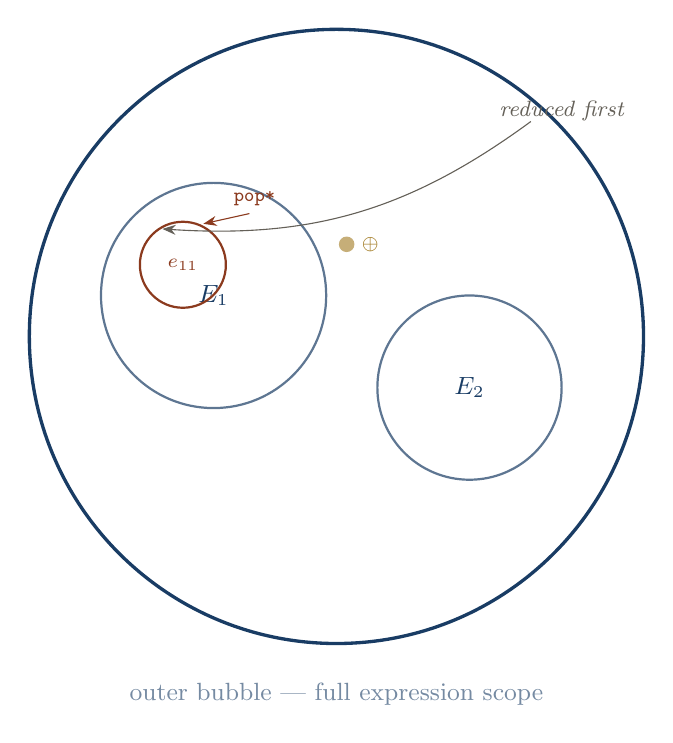
\begin{tikzpicture}[scale=1.3, >=Stealth]

  % --- outer bubble ---
  \draw[spblue, very thick] (0,0) circle (3);
  \node[font=\small, text=spblue!60] at (0,-3.5)
    {outer bubble — full expression scope};

  % --- left inner bubble ---
  \draw[spblue!70, thick] (-1.2, 0.4) circle (1.1);
  \node[font=\small, text=spblue] at (-1.2, 0.4) {$E_1$};

  % --- right inner bubble ---
  \draw[spblue!70, thick] (1.3,-0.5) circle (0.9);
  \node[font=\small, text=spblue] at (1.3,-0.5) {$E_2$};

  % --- deepest bubble inside left ---
  \draw[sprust, thick] (-1.5, 0.7) circle (0.42);
  \node[font=\scriptsize, text=sprust] at (-1.5, 0.7) {$e_{11}$};

  % --- pop* marker on innermost ---
  \node[font=\scriptsize\bfseries, text=sprust]
    at (-0.8, 1.35) {\texttt{pop*}};
  \draw[->, sprust, thin] (-0.85,1.2) -- (-1.3, 1.1);

  % --- arrows showing evaluation order (inner first) ---
  \node[font=\footnotesize\itshape, text=spgray] at (2.2, 2.2)
    {reduced first};
  \draw[->, thin, spgray] (1.9, 2.1) to[bend left=20] (-1.7,1.05);

  % --- operator token at centre ---
  \filldraw[spgold!60] (0.1, 0.9) circle (2pt);
  \node[right, font=\scriptsize, text=spgold] at (0.15, 0.9)
    {$\oplus$};

\end{tikzpicture}
\caption{\textbf{Spherepop expressions as nested bubbles.}
  Nesting depth encodes evaluation priority: the innermost bubble
  is the first commitment site (\texttt{pop*}). Structure is transient;
  it is consumed during reduction and does not persist in the trace.}
\label{fig:bubbles}
\end{figure}


\section{Reduction Rules and Sequences}
\label{sec:sp:reduction}

\begin{definition}[Reduction]
\label{def:sp-reduction}
Let $\ruleR$ be a set of local rewrite rules of the form
$(E_1 \cdots E_n) \to E'$,
where $E'$ is an expression. A \emph{reduction step} consists in selecting a
bubble within an expression and replacing it according to a rule in $\ruleR$.
A \emph{reduction sequence} is a finite chain
$E_0 \to E_1 \to \cdots \to E_k$
in which each step applies a rule to some bubble of the preceding expression.
\end{definition}

Reduction in Spherepop is strictly local. At each step, a single bubble is
selected and replaced. The global behaviour of evaluation emerges from the
composition of these local operations.

Crucially, each reduction step eliminates a portion of the expression. The
original bubble is not retained alongside its replacement. The system does not
maintain a record of alternatives or preserve prior states. Each step
constitutes a commitment that restricts the space of possible future reductions.

\section{Normal Forms and the Evaluation Map}
\label{sec:sp:normalforms}

\begin{definition}[Normal Form and Evaluation Map]
\label{def:sp-normalform}
An expression $E$ is said to be in \emph{normal form} if no rule in $\ruleR$
applies to any of its subexpressions.
\end{definition}

\begin{assumption}[Confluence and Termination]
\label{asm:confluence}
The rule set $\ruleR$ is terminating and confluent: every expression $E$
reduces to a unique normal form regardless of the order in which rules are
applied.
\end{assumption}

Under this assumption, the \emph{evaluation map}
$\evalf : \Expr \to \NF$
assigns to each expression its unique normal form, denoted
$\trace(E) = \evalf(E)$.
The map $\evalf$ is surjective (every normal form evaluates to itself) and
idempotent ($\evalf(\evalf(E)) = \evalf(E)$); it is therefore a canonical
surjective projection from $\Expr$ onto $\NF$, inducing the quotient
$\NF \cong \Expr/{\tequiv}$.

Termination ensures that every reduction sequence reaches a state to which no
further rules apply. Confluence ensures this state is independent of the
sequence chosen. Without confluence, identity becomes path-dependent: two
trajectories from the same expression could reach distinct normal forms,
fracturing the notion of trace. We treat confluence not as a technical
convenience but as the condition under which a well-defined notion of identity
is available at all. Non-confluent systems yield path-dependent identity theory,
which we set aside as a distinct direction.

\section{Append-Only Dynamics}
\label{sec:sp:appendonly}

The defining feature of the Spherepop calculus is that reduction is
append-only. Each step in a reduction sequence contributes to a history of
commitments, but none of these commitments can be withdrawn.

A reduction sequence $E_0 \to E_1 \to \cdots \to E_k$ is not merely a path
between two expressions, but an ordered record of transformations. At each
step, the set of admissible continuations is restricted. Once a bubble has been
reduced, the alternatives it represented are no longer available.

\paragraph{Analogy.}
A notarised deed transfer operates on the same principle. Once signed, witnessed, and recorded, the transfer is entered into the land register as a permanent and irrevocable entry. The alternative futures in which the seller retained the property---or sold to a different buyer---are not merely set aside; they are legally eliminated. The land register is an append-only ledger, and no subsequent entry can remove a prior one. Spherepop reduction is formally identical: each reduction step is a notarisation of a decision that forecloses alternatives and can never be undone.

In this sense, reduction does not explore a space of possibilities; it contracts
that space. The evaluation process progressively eliminates incompatible
structures until a terminal configuration is reached. The normal form is not
one possibility among many equally accessible alternatives. It is what remains
after all incompatible possibilities have been excluded.

%------------------------------------------------------------------
% FIG 4 — Collapse Funnel / Contraction of Possibility Space (Ch 3–4)
%------------------------------------------------------------------
\begin{figure}[htbp]
\centering
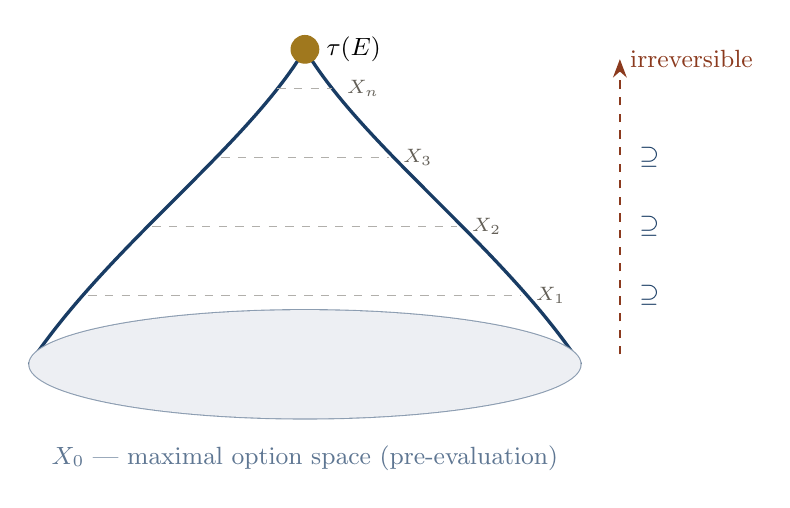
\begin{tikzpicture}[scale=1.25, >=Stealth]

  % --- funnel outline (two bezier curves meeting at apex) ---
  \draw[spblue, very thick]
    (-2.8, 0) .. controls (-2.0,1.2) and (-0.6,2.2) .. (0, 3.2);
  \draw[spblue, very thick]
    ( 2.8, 0) .. controls ( 2.0,1.2) and ( 0.6,2.2) .. (0, 3.2);

  % --- base ellipse (high entropy) ---
  \draw[spblue!50, thick] (0,0) ellipse (2.8 and 0.55);
  \fill[spblue!8] (0,0) ellipse (2.8 and 0.55);

  % --- horizontal slices (option spaces X_k) ---
  \foreach \h/\r/\lbl in {
    0.7/2.2/$X_1$,
    1.4/1.55/$X_2$,
    2.1/0.85/$X_3$,
    2.8/0.28/$X_n$}
  {
    \draw[spgray!50, dashed] (-\r, \h) -- (\r, \h);
    \node[right, font=\scriptsize, text=spgray] at (\r+0.05, \h) {\lbl};
  }

  % --- inclusion annotations ---
  \node[font=\small, text=spblue] at (3.5, 0.7) {$\supseteq$};
  \node[font=\small, text=spblue] at (3.5, 1.4) {$\supseteq$};
  \node[font=\small, text=spblue] at (3.5, 2.1) {$\supseteq$};

  % --- bottom label ---
  \node[font=\small, text=spblue!70] at (0,-0.95)
    {$X_0$ — maximal option space (pre-evaluation)};

  % --- apex: trace ---
  \filldraw[spgold] (0, 3.2) circle (4pt);
  \node[right, font=\small\bfseries] at (0.12, 3.2)
    {$\trace(E)$};

  % --- arrow of time ---
  \draw[->, thick, sprust, dashed]
    (3.2, 0.1) -- (3.2, 3.1)
    node[right, font=\small, text=sprust] {irreversible};

\end{tikzpicture}
\caption{\textbf{Irreversible contraction of the option space.}
  Each reduction step yields $X_{k+1} \subseteq X_k$ (strict inclusion when
  new constraints eliminate possibilities).
  The sequence terminates at the trace, which carries no record of the
  path that produced it.}
\label{fig:funnel}
\end{figure}


This interpretation distinguishes Spherepop from standard rewriting systems in
which reduction sequences may be viewed abstractly as interchangeable paths
between equivalent expressions. In Spherepop, the path itself has ontological
significance. It records the sequence of eliminations by which the final result
was obtained.

\section{From Expressions to Histories}
\label{sec:sp:history}

The preceding considerations suggest a shift in how expressions are understood.
An expression is not merely a static object to which rules are applied, but the
starting point of a reduction trajectory. Its identity is not exhausted by its
syntactic form, but includes the history of transformations it undergoes.

At the same time, this history is not preserved in the final result. The normal
form retains only what survives the process of elimination. Distinct histories
may converge to the same terminal state, and the differences between them are
not recoverable from that state.

This tension between the richness of the reduction history and the minimality
of the normal form is the central structural feature of the calculus. It is
this feature that gives rise to the loss of preimage and, ultimately, to the
need to redefine identity. In the next chapter, this observation is formalised.
The evaluation map is shown to lack a right inverse, and the resulting notion
of collapse provides the hinge on which the remainder of the theory turns.


\section{Equivalence to the Lambda Calculus and Turing Completeness}
\label{sec:sp:lambda}

The Spherepop calculus is not merely analogous to classical models of
computation; it is computationally equivalent to them. We establish this by
constructing explicit translations between Spherepop and the untyped lambda
calculus, from which Turing completeness follows as a corollary.

\subsection{Translating Lambda Terms into Spherepop}

Recall that every untyped lambda term is one of three forms: a variable $x$,
an abstraction $\lambda x.\, M$, or an application $M\, N$. We define a
translation $\llbracket \cdot \rrbracket : \Lambda \to \Expr$ by structural
induction:
\begin{align*}
  \llbracket x \rrbracket
    &= x, \\
  \llbracket \lambda x.\, M \rrbracket
    &= (\mathtt{lam}\; x\; \llbracket M \rrbracket), \\
  \llbracket M\, N \rrbracket
    &= (\llbracket M \rrbracket\; \llbracket N \rrbracket).
\end{align*}
Variables translate to atomic tokens. Abstraction becomes a labelled bubble
carrying the variable name and the translated body. Application becomes a
binary bubble whose first child is the translated function and whose second
child is the translated argument.

Beta-reduction in the lambda calculus, $(\lambda x.\, M)\, N \to M[N/x]$,
corresponds to a single Spherepop reduction step: the outermost application
bubble is popped, the variable $x$ throughout the body $M$ is replaced by
the argument $\llbracket N \rrbracket$, and the enclosing structure is
discarded. This substitution rule is straightforwardly encoded in $\ruleR$.
The translation therefore respects reduction: if $M \to_\beta M'$ then
$\llbracket M \rrbracket \to_{\ruleR} \llbracket M' \rrbracket$.

\subsection{Translating Spherepop into the Lambda Calculus}

In the opposite direction, define $\lceil \cdot \rceil : \Expr \to \Lambda$
by treating every Spherepop bubble $(E_1 \cdots E_n)$ as a left-associated
application:
\[
  \lceil (E_1 \cdots E_n) \rceil
  = \lceil E_1 \rceil\; \lceil E_2 \rceil\; \cdots\; \lceil E_n \rceil,
\]
where nesting is handled by structural recursion. A bubble with a single
element is the identity applied to its content. Named operators such as
$\mathtt{lam}$, $\mathtt{pop}$, $\bind$, and $\refuse$ are encoded as
specific closed lambda terms (combinators) using the standard Church
encoding of data and control structures.

The key point is that the core Spherepop operations---substitution during
a pop step, constraint propagation in bind, and the monotone contraction of
option spaces---all have direct lambda encodings. This follows from the
universality of the lambda calculus: any computable function can be expressed
as a lambda term \cite{church1941}.

\subsection{Confluence and Normal Forms}

The Spherepop calculus satisfies Assumption~\ref{asm:confluence} for the
relevant class of reduction rules, corresponding to the fact that
beta-normal forms exist and are unique for strongly normalising lambda terms.
For non-terminating computations, the normal form is undefined in both
systems, preserving the correspondence exactly.

\begin{theorem}[Computational Equivalence]
\label{thm:turing-complete}
The Spherepop calculus is computationally equivalent to the untyped lambda
calculus, and therefore to Turing machines. Specifically:
\begin{enumerate}[label=(\roman*)]
  \item Every lambda term can be simulated by a Spherepop expression, and
    beta-reduction corresponds to Spherepop reduction steps.
  \item Every Spherepop expression has a faithful encoding as a lambda term,
    and Spherepop reduction is simulated by beta-reduction.
  \item A function is Spherepop-computable if and only if it is
    Turing-computable.
\end{enumerate}
\end{theorem}

\begin{proof}[Proof (Sketch)]
Parts (i) and (ii) follow from the translations $\llbracket\cdot\rrbracket$
and $\lceil\cdot\rceil$ constructed above, which preserve reduction steps in
each direction. Part (iii) follows from the Church--Turing thesis and the
known equivalence of the untyped lambda calculus and Turing machines
\cite{barendregt1984}: any Turing-computable function is lambda-definable,
and any lambda-definable function is Turing-computable. Since Spherepop
simulates the lambda calculus and is simulated by it, the class of
Spherepop-computable functions coincides with the class of Turing-computable
functions. \qed
\end{proof}

\subsection{What Turing Completeness Does and Does Not Establish}

The equivalence result is important for two reasons. First, it ensures that
Spherepop is not a toy calculus but a full model of computation: any
algorithm can be expressed in it. Second, it grounds the irreversibility
analysis in a setting the reader already understands: lambda reduction is
also irreversible in the relevant sense. Beta-reduction destroys the
redex---the source structure---and the result does not encode which redex
produced it.

However, Turing completeness does not explain irreversibility; it presupposes
it. The point of the present work is not to establish that Spherepop can
compute everything a Turing machine can (though it can), but to analyse what
it means for an evaluation to be irreversible, and to develop a theory of
identity appropriate to that condition. The Turing equivalence confirms that
this analysis applies to the full generality of computable processes.

%=============================================================
\part{The Hinge: Collapse and Its Consequences}
%=============================================================

%-------------------------------------------------------------
\chapter{Collapse and the Loss of Preimage}
\label{ch:collapse}
%-------------------------------------------------------------

The Spherepop calculus makes explicit a structural feature that is only implicit
in ordinary computation: evaluation eliminates information. The reduction of an
expression to its normal form preserves certain invariants while discarding the
structure that produced them. This asymmetry between what is retained and what
is lost is the defining property of collapse.

In this chapter, that asymmetry is formalised. We show that the evaluation map
does not admit a right inverse, and we analyse the resulting structure in terms
of equivalence classes of expressions. The loss of preimage is not an accidental
limitation of particular reduction sequences, but a necessary consequence of the
many-to-one character of evaluation.

\begin{tcolorbox}[hinge, title={Part II Hinge}]
  \textbf{Collapse has no right inverse.} This is the structural asymmetry that
  makes classical self-reference fail and forces the redefinitions in Parts~III
  and~IV.
\end{tcolorbox}

\section{Prerequisites}

This chapter assumes the definitions of Chapter~3 (expressions, bubbles, reduction rules, evaluation map) and familiarity with basic set-theoretic notions: functions, surjectivity, and equivalence relations. The proof of Proposition~4.1 uses a simple fiber argument requiring no machinery beyond elementary combinatorics. Readers with a background in abstract algebra will recognise the quotient construction immediately; those without should find the prose development of the quotient $\Expr/{\tequiv}$ self-contained.

\section{The Absence of a Right Inverse}
\label{sec:collapse:noinverse}

\begin{definition}[Right Inverse]
\label{def:right-inverse}
A function $g : \NF \to \Expr$ is a \emph{right inverse} of the evaluation map
$\evalf : \Expr \to \NF$ if $\evalf \circ g = \mathrm{id}_{\NF}$.
\end{definition}

The existence of a right inverse would imply that every normal form contains
sufficient information to reconstruct at least one expression evaluating to it.
The following proposition shows this is not the case.

\begin{proposition}[Non-Existence of Right Inverse]
\label{prop:no-right-inverse}
The evaluation map $\evalf : \Expr \to \NF$ admits no right inverse.
\end{proposition}

\begin{proof}
Assume for contradiction that there exists a function $g : \NF \to \Expr$ such
that $\evalf(g(N)) = N$ for all $N \in \NF$.

Consider a normal form $N$ that admits multiple distinct preimages. Such cases
arise immediately. Let $E_1 = (8 + (3 \times 5))$ and $E_2 = (8 + 15)$. Both
expressions reduce to $\evalf(E_1) = \evalf(E_2) = 23$, so $E_1, E_2 \in
\preimgset{23}$, yet $E_1 \neq E_2$.

The function $g$ must assign a single expression $g(23)$ whose evaluation
yields $23$. However, the value $23$ does not encode any information that
distinguishes $E_1$ from $E_2$. Any choice of $g(23)$ therefore depends on
information not contained in $23$ itself. Since this reasoning applies to every
normal form with multiple preimages, no function $g$ can be defined solely in
terms of $\NF$ such that $\evalf \circ g = \mathrm{id}_{\NF}$.
\qed
\end{proof}

\begin{remark}
The evaluation map $\evalf$ is therefore a canonical quotient map identifying
all expressions in a fiber with a single invariant representative. The absence
of a right inverse is not a deficiency but a structural consequence: the
quotient point $N \in \NF$ does not encode which preimage produced it.
\end{remark}

\section{Preimage and Trace}
\label{sec:collapse:preimage}

\begin{definition}[Preimage and Trace]
\label{def:preimage-trace}
Let $N \in \NF$. The \emph{preimage} of $N$ is the set
$\preimgset{N} = \{ E \in \Expr \mid \evalf(E) = N \}$.
For any expression $E$, the \emph{trace} of $E$ is its normal form
$\trace(E) = \evalf(E)$.
\end{definition}

The preimage of a normal form collects all expressions that collapse to the
same terminal state. The trace is the only information that survives evaluation.
While the preimage may be large and structurally diverse, the trace is a single
object that does not retain the distinctions present in the preimage.

The absence of a right inverse implies that the preimage cannot be recovered
from the trace. The trace is therefore not a compressed encoding of the
preimage, but a projection that discards its internal differences entirely.

%------------------------------------------------------------------
% FIG 1 — Preimage / Fiber Collapse (Chapter 4 hinge)
%------------------------------------------------------------------
\begin{figure}[htbp]
\centering
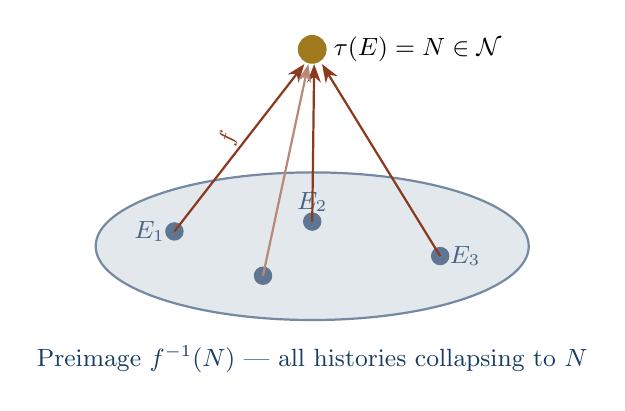
\begin{tikzpicture}[scale=1.25, >=Stealth]

  % --- lower fiber ellipse (shaded "cloud") ---
  \begin{scope}[shift={(0,0)}]
    \fill[spblue!12] (0,0) ellipse (2.2 and 0.75);
    \draw[spblue!60, thick] (0,0) ellipse (2.2 and 0.75);
  \end{scope}

  % --- sample preimage points ---
  \filldraw[spblue!70] (-1.4, 0.15) circle (2.5pt)
    node[left, font=\small, text=spblue!80] {$E_1$};
  \filldraw[spblue!70] ( 0.0, 0.25) circle (2.5pt)
    node[above, font=\small, text=spblue!80] {$E_2$};
  \filldraw[spblue!70] ( 1.3,-0.10) circle (2.5pt)
    node[right, font=\small, text=spblue!80] {$E_3$};
  \filldraw[spblue!70] (-0.5,-0.30) circle (2.5pt);

  % --- label for fiber ---
  \node[font=\small, text=spblue] at (0,-1.15)
    {Preimage $f^{-1}(N)$ — all histories collapsing to $N$};

  % --- convergence arrows ---
  \draw[->, thick, sprust]   (-1.4, 0.15) -- (-0.08, 1.85);
  \draw[->, thick, sprust]   ( 0.0, 0.25) -- ( 0.02, 1.85);
  \draw[->, thick, sprust]   ( 1.3,-0.10) -- ( 0.10, 1.85);
  \draw[->, thick, sprust!60](-0.5,-0.30) -- (-0.04, 1.85);

  % --- trace point ---
  \filldraw[spgold] (0, 2.0) circle (4pt);
  \node[right, font=\small\bfseries] at (0.12, 2.0)
    {$\trace(E) = N \in \NF$};

  % --- evaluation label on arrow ---
  \node[rotate=75, font=\footnotesize\itshape, text=sprust]
    at (-0.85, 1.1) {$\evalf$};

\end{tikzpicture}
\caption{\textbf{Many-to-one collapse.}
  A fiber of expressions contracts irreversibly to a single trace.
  The preimage is not recoverable from~$N$; this is the fundamental
  asymmetry established by Proposition~4.1.}
\label{fig:collapse}
\end{figure}


\section{The Quotient Structure of Collapse}
\label{sec:collapse:topology}

The evaluation map induces an equivalence relation on $\Expr$:
\[
  E \tequiv E' \;\Longleftrightarrow\; \evalf(E) = \evalf(E').
\]
Two expressions are equivalent precisely when they collapse to the same trace.
This equivalence partitions $\Expr$ into disjoint classes, each class
consisting of all expressions that share a common normal form. The set of
normal forms $\NF$ can therefore be identified with the quotient
$\Expr / {\tequiv}$.

Under this identification, the evaluation map $\evalf$ is the canonical
projection sending each expression to its equivalence class. Each fiber
$\preimgset{N}$ is collapsed to a single representative $N$.

The essential asymmetry is now clear. The projection $\evalf$ is many-to-one.
Each equivalence class contains multiple histories, but the quotient retains
only a single invariant. The distinctions between elements of a fiber are not
hidden; they are eliminated as distinguishable structure. Collapse is therefore
not merely a loss of detail, but a structural operation that identifies all
histories compatible with a single invariant outcome.

\paragraph{Analogy.}
A photograph is a quotient. The light entering the lens during the exposure represents a large and diverse set of physical configurations---the precise trajectory of every photon, the exact state of every surface in the scene. All of this is collapsed onto a flat image. Two physically distinct scenes that differ only in ways to which the sensor is insensitive yield identical photographs. The photograph is the trace; the original scene is the preimage. No darkroom technique recovers the preimage from the print. What is lost in the exposure is lost permanently, and the photograph carries no record of how many distinct scenes could have produced it.

\section{Irreversibility as Structural Asymmetry}
\label{sec:collapse:asymmetry}

The non-existence of a right inverse establishes a fundamental asymmetry between
expressions and their traces. While every expression determines a unique trace,
no trace determines a unique expression.

This asymmetry is not contingent on the particular choice of reduction rules. It
follows from the basic form of evaluation as a process that replaces structured
objects with simpler ones. Whenever distinct structures reduce to a common
result, the information distinguishing them is irretrievably lost. Irreversibility
is therefore not an empirical limitation but a structural fact. The evaluation
map contracts the space of expressions onto a space of invariants, and this
contraction cannot be undone.

%-------------------------------------------------------------
\chapter{Identity as Event History}
\label{ch:identity}
%-------------------------------------------------------------

The preceding chapter established that evaluation eliminates the information
required to reconstruct the origin of an expression. Distinct expressions may
collapse to the same trace, and the trace does not encode the structure of its
preimage. This result forces a revision of the notion of identity.

In reversible systems, identity is typically defined in terms of state. An
object is identified either by its syntactic structure or by its position within
a space of configurations. Such definitions presuppose that the relevant
structure is preserved or recoverable. Under irreversible collapse, this
presupposition fails.

In this chapter, identity is relocated from the domain of initial structure to
the domain of what survives evaluation. The trace becomes the carrier of
identity, while the history of evaluation provides the context in which that
identity is realised.

\section{Prerequisites}

This chapter builds directly on Chapter~4. The reader should understand the non-existence of a right inverse and the resulting quotient structure before proceeding. Some familiarity with philosophy of identity is helpful for the motivating discussion in Section~5.1, but is not required for the formal content. The definition of the event word ($\partial(E) \in \Sigma^*$) assumes basic acquaintance with formal languages and the monoid of finite strings.

\section{The Failure of State-Based Identity}
\label{sec:identity:failure}

In a reversible setting, a state may be taken to determine its history, at
least up to equivalence. This allows identity to be defined extensionally: two
objects are identical if they occupy the same state or share the same structure.

In an irreversible system, a state no longer determines its origin. The
evaluation map $\evalf$ identifies distinct expressions at the level of their
trace, and the information distinguishing those expressions is not recoverable.
A normal form therefore underdetermines the histories that produced it.

It follows that identity cannot be grounded in the initial configuration of an
expression. Any criterion that depends on reconstructing the preimage is
inapplicable. Identity must instead be located in what remains after collapse.

\section{Event Words}
\label{sec:identity:eventword}

\begin{definition}[Event Word]
\label{def:event-word}
Let $\Sigma$ be the set of atomic reduction events. The \emph{event word} of an
expression $E$ is the sequence $\eventword(E) \in \Sigma^*$ that records the
ordered reduction steps transforming $E$ into its normal form.
\end{definition}

The event word captures the history of evaluation as a sequence of commitments.
Each symbol represents a local transformation, and the concatenation of these
symbols records the trajectory by which the expression is reduced. This history
is richer than the final result. Distinct event words may correspond to
expressions that collapse to the same trace. The event word therefore carries
information that is not preserved under evaluation.

\section{Trace and Identity}
\label{sec:identity:defn}

\begin{definition}[Trace Identity]
\label{def:identity}
The \emph{identity} of an expression $E$ under irreversible reduction is the
equivalence class
$[E]_{\tequiv} = \{ E' \in \Expr \mid \trace(E') = \trace(E) \}$.
Two expressions are \emph{co-identical} if they share the same trace.
\end{definition}

This equivalence is the coarsest congruence on $\Expr$ preserved by $\evalf$:
any finer distinction between expressions is eliminated by evaluation, so no
finer identity criterion remains observable. Since no distinction finer than
trace survives evaluation, trace equivalence is the maximal invariant available
to the system.

Identity is thus defined in terms of the invariant that survives evaluation.
While the event word records the path taken, the trace records the outcome that
remains once all incompatible possibilities have been eliminated.

\paragraph{Analogy.}
Two witnesses to the same accident recall different sequences of detail---one noticed the colour of a car first, the other the sound of the impact. Their memories are different event words. Yet both agree on what happened: the essential facts that constitute the identity of the event are the same in both accounts. Those shared facts are the trace. The divergent details of the individual recollections are elements of the same preimage fiber: different paths that collapsed to the same invariant. The event itself is defined not by either witness's private sequence of impressions, but by what is common to all accounts that agree on its identity. This definition
reflects the structural asymmetry established in the previous chapter. Since the
preimage cannot be recovered, identity cannot depend on it. The only stable
criterion is the trace.

\section{Event History and Invariance}
\label{sec:identity:history}

The event word and the trace carry orthogonal information. The event word records
the history of commitments and distinguishes trajectories that may converge to
the same result. The trace records only the surviving invariant and identifies
trajectories that differ but collapse to the same endpoint.

Thus $\eventword(E) \neq \eventword(E')$ does not imply $\trace(E) \neq
\trace(E')$, and conversely, shared traces do not entail shared histories. The
event word is path-sensitive; the trace is path-invariant. Identity, under
irreversibility, attaches to the latter. Event words record how a trace was
reached; they do not determine identity. Identity is defined solely at the
level of the trace. This shows that identity is not a
property of the path taken, but of the endpoint reached.

\section{Mereological Inclusion}
\label{sec:identity:mereology}

The event word also induces a notion of inclusion. If the reduction sequence of
one expression forms a subsequence of the reduction sequence of another, then
the first may be regarded as a part of the second in a historical sense.

This relation aligns with the containment of bubbles in Spherepop expressions.
Nested structures give rise to nested segments of the event word, and the
elimination of a substructure corresponds to the contraction of a segment of
the history. Mereological inclusion is therefore not defined in terms of static
substructure, but in terms of containment within a history of transformations.

\section{Identity After Collapse}
\label{sec:identity:conclusion}

The relocation of identity from structure to trace has a decisive consequence.
An expression is no longer identified by what it was, but by what it becomes
under evaluation. Identity is not preserved through the process of reduction;
it is established by that process. The elimination of structure is not a loss
to be compensated, but the mechanism by which invariant identity emerges. In
this sense, identity is not a precondition of evaluation, but its result.

\section{Regions as Possible Worlds: The Categorical Geometry of Scope}
\label{sec:identity:worlds}

The nested bubble structure of Spherepop expressions is not merely a notational
device. It is a model of \emph{scope}: each bubble delimits a bounded region
within which certain operations and tokens are active, and outside which they
are not. This structure has a precise interpretation in category theory and
connects the formalism to a deep philosophical tradition about possible worlds
and the nature of models.

\subsection{Bubbles as Objects in a Presheaf Category}

In the internal logic of a topos, an object $A$ in a category $\mathbf{C}$ can
be interpreted as a collection of \emph{local data} varying across contexts.
A context here is an object of $\mathbf{C}$ itself---a ``stage of definition''
or a bounded region of applicability. Morphisms between contexts correspond to
restrictions: data available in a larger context restricts to data available
in a smaller one.

Spherepop bubbles instantiate exactly this structure. Each bubble $B$ is a
context: the tokens and operators it contains are in scope within $B$ and
are not directly visible outside it. A nested bubble $B'$ inside $B$
corresponds to a subcontext---a more restricted stage of definition---and the
reduction rules that pop $B'$ before $B$ correspond to the restriction
functors that resolve inner contexts before outer ones.

Formally, the collection of all bubbles in an expression, ordered by containment,
forms a partial order $(\mathcal{B}, \sqsubseteq)$. This partial order is the
base of the presheaf of histories constructed in Appendix~C: the data assigned
to each bubble is the set of all compatible reduction sequences whose scope
falls within that bubble. Restriction maps send a global reduction to its
local trace within a subbubble.

\subsection{Scope Order as a Model of the World}

When a human being sets out to understand a situation---whether by writing
a program, constructing a scientific model, or parsing an utterance---the
fundamental cognitive operation is the \emph{establishment of scope}. One
defines a boundary within which certain entities are active, certain relations
hold, and certain operations are admissible. Outside that boundary, different
rules apply.

This is exactly the operation performed by bubble introduction in Spherepop.
A new bubble does not add tokens arbitrarily; it introduces a bounded context
with its own evaluation rules. The tokens within it are not yet committed to
any global configuration---they are a local possibility space waiting to be
resolved. In this sense, a bubble is a \emph{local world}: a region of
structured possibility that will eventually be popped into the global trace.

The order in which bubbles are introduced and popped corresponds to the order
in which partial models are built and collapsed. A deeply nested bubble
represents a fine-grained local commitment made before its containing context
has been resolved. A shallow bubble represents a coarser constraint whose
resolution depends on prior inner work. This nesting structure is isomorphic
to the nested quantifier scopes and dependent type contexts of formal logic,
and to the nested frames and activation records of a call stack in programming
languages.

\subsection{Humans as Scope-Establishing Agents}

The act of constructing a mental model---of a physical situation, a
grammatical sentence, a social interaction, or a mathematical proof---is
structurally identical to the act of introducing a bubble. The modeller
establishes a scope: which entities are present, which relations hold, which
operations are admissible within this representation. The model is then
evaluated---resolved, tested against constraints, reduced to its salient
content---and the scaffolding of its construction is discarded.

The analogy is not metaphorical. In Chapter~11, the H-LFG parse of an
utterance shows exactly this process: each lexical event introduces a
bounded local constraint (the bubble of a nominal phrase, the scope of a
verb), and the global f-structure is the trace that remains after all local
scaffolding has been consumed. The listener builds a model of the sentence by
establishing and collapsing scopes in the order dictated by the linear sequence
of lexical events.

At a broader scale, scientific modelling follows the same pattern. A model is
a bubble---a bounded context with its own ontology---within which certain
idealisations hold and others do not. The model is evaluated against data,
and the aspects of reality it cannot accommodate are the points at which its
constraints become incompatible with the external option space. A model that
survives this evaluation is grammatical in the H-LFG sense: it has a non-empty
trace. A model that cannot accommodate the data is ungrammatical: total
collapse.

\subsection{Regions in Categorical Semantics}

In the categorical semantics of modal and possible-worlds logic, a \emph{world}
is an object $w$ in a Kripke frame---a directed graph whose edges represent
the accessibility relation between worlds. A proposition $\varphi$ is true at
world $w$ if it is satisfied by the local data at $w$. The global truth of
$\varphi$ is determined by whether it holds in all worlds accessible from
the current one.

The partial order $(\mathcal{B}, \sqsubseteq)$ of bubbles is a Kripke frame
in which containment is the accessibility relation: a bubble $B'$ is
accessible from $B$ (i.e., $B' \sqsubseteq B$) if $B'$ is contained within
$B$. A token is \emph{in scope at} $B$ if it is contained within $B$ and not
yet popped. The evaluation of the innermost bubble first corresponds to
computing truth values at the most accessible worlds before resolving the
question at the containing world.

This is not a loose analogy. The sheaf of histories over $(\NF, \preceq)$
constructed in Appendix~C is the precise categorical expression of this
structure. Local sections correspond to locally consistent valuations at
individual worlds; global sections correspond to globally consistent models.
The failure of gluing---ungrammaticality---corresponds to the impossibility
of finding a model that satisfies all local constraints simultaneously, which
is precisely the categorical definition of unsatisfiability in the internal
logic of the sheaf.

\subsection{Scope, Commitment, and the Arrow of Time}

The order in which bubbles are introduced and popped defines a direction of
time within the computation. Inner bubbles precede outer ones; local
commitments precede global ones. This order is not arbitrary---it is the
order in which the world of the expression is constructed and then dismantled.

In this light, the append-only dynamics of Spherepop reduction formalises a
deep feature of cognition and action: to act is to commit to a scope, and to
commit is to foreclose alternatives. The space of possible worlds narrows with
each commitment. Identity---in computation, in language, in thought---is what
remains when all possible worlds except one have been eliminated.


%-------------------------------------------------------------
\chapter{Logical Stratification Under Collapse}
\label{ch:priest}
%-------------------------------------------------------------

\begin{tcolorbox}[priest, title={Priest Integration}]
  The introduction of an irreversible evaluation operator $\evalf$
  \emph{induces} a stratification of logical interpretation. The distinction
  between theory, practice, and fact is no longer optional---it is
  \emph{structurally necessary}.
\end{tcolorbox}

\section{Prerequisites}

This chapter assumes Chapters~3 through~5. On the philosophical side, some acquaintance with the philosophy of logic is helpful, though Priest\textquoteright s distinction between \docens{}, \utens{}, and \ens{} is explained from scratch. Readers unfamiliar with paraconsistent or non-classical logic need not have prior exposure; those ideas are developed further in Chapter~13. The mathematical content of this chapter (the Correspondence Theorem and the Lemma on Trace Adequacy) requires only the definitions already established.

\section{Priest's Tripartite Distinction}
\label{sec:priest:three}

In ``Revising Logic,'' Graham Priest distinguishes three senses in which we
speak of logic. \Docens{} is the formal theory of valid inference, as codified
in textbooks. Revision at this level proceeds by the standard criteria of theory
choice: simplicity, fruitfulness, adequacy to data. \Utens{} is the norms
governing actual inferential practice, once systematic errors are corrected.
Priest argues that it is rational to revise \utens{} by bringing practice into
accord with the best available \docens{}. \Ens{} is the facts of validity
themselves---what actually follows from what, independently of our theoretical
attempts to capture it.

Much confusion about logical revision arises, Priest contends, from conflating
these levels. A revision of \docens{} need not be a revision of \ens{}; a change
in \utens{} need not wait for a change in \ens{}.

\section{The Spherepop Correspondence}
\label{sec:priest:correspondence}

The Spherepop calculus provides a setting in which Priest's three levels are not
only distinguishable but are identified with distinct mathematical objects.

\begin{theorem}[Correspondence of Collapse]
\label{thm:correspondence}
  The irreversible reduction operator $\evalf$ induces a tripartite
  correspondence:
  \begin{align*}
    \docens{} &\;\longleftrightarrow\; (\Expr,\, \ruleR), \\
    \utens{}  &\;\longleftrightarrow\; \text{reduction trajectories in }
                \Expr, \\
    \ens{}    &\;\longleftrightarrow\; \evalf(\Expr) \subseteq \NF.
  \end{align*}
  These are not equivalent representations but distinct strata connected by
  the evaluation process.
\end{theorem}

\begin{remark}
This stratification is not interpretive but induced: the irreversibility of
$\evalf$ severs theory, practice, and outcome into distinct mathematical
objects.

\paragraph{Analogy.}
Consider a musical score, a performance, and the acoustic event that reaches the audience. The score is logica docens: a formal specification of admissible realisations. The performer's practice---the choices of tempo, dynamics, and articulation in real time---is logica utens: the actual sequence of irreversible commitments that instantiate one trajectory from the score's option space. The acoustic trace that the audience hears, which cannot be retracted once produced, is logica ens: the terminal fact. A recording of the performance is not the score; the score is not the performance; and neither is identical to the acoustic event that has already collapsed into the listener's memory. Irreversibility is what separates them. In reversible systems the three strata coincide because the formal
system determines outcomes and outcomes determine preimages. Irreversibility
dissolves both identifications simultaneously.
\end{remark}

\begin{proof}
The formal calculus $(\Expr, \ruleR)$ is a specification of admissible
transformations---a theory---and corresponds to \docens{}. A reduction
trajectory $E_0 \to E_1 \to \cdots \to E_k$ is a sequence of actual
commitments, the practice of evaluation, and corresponds to \utens{}. By
confluence, distinct trajectories over the same expression converge to the same
terminal object; that terminal object is invariant across all paths in the fiber
and corresponds to \ens{}: the fact of what the expression evaluates to,
independent of route. \qed
\end{proof}

\section{Divergence Under Irreversibility}
\label{sec:priest:divergence}

In reversible systems, the three levels are implicitly conflated: the formal
theory specifies a recoverable transformation, so \docens{} and \ens{}
coincide, and \utens{} is merely the execution of that specification. In
Spherepop, this conflation is impossible.

\begin{proposition}[Divergence of Logical Strata]
\label{prop:divergence}
  In the Spherepop calculus, \docens{}, \utens{}, and \ens{} are pairwise
  non-equivalent: syntactically distinct expressions may share a trace, so
  \docens{} does not determine \ens{}; distinct trajectories may realise the
  same trace, so \utens{} does not determine \docens{}; and the trace is
  determined by the fiber structure of $\evalf$, not by syntactic form or
  trajectory alone, so \ens{} is not reducible to either of the others.
\end{proposition}

\section{Validity as Trace Stability}
\label{sec:priest:validity}

The standard notion of validity concerns truth-preservation under substitution.
In an irreversible calculus, this must be revised.

\begin{definition}[Trace Validity]
\label{def:trace-validity}
  An inference from $E$ to $E'$ is \emph{trace-valid} if
  $\trace(E) \tequiv \trace(E')$.
\end{definition}

This relocates validity from \docens{} (syntactic preservation) to \ens{}
(stability of trace under projection). It is a revision in Priest's sense:
we have identified a new adequacy criterion and updated both theory and practice
accordingly.

\begin{lemma}[Trace Adequacy]
\label{lem:trace-adequacy}
  In an irreversible calculus, the only observable invariant is the trace
  $\trace(E)$. Therefore any criterion of correctness must be defined over
  $\NF$, not over $\Expr$.
\end{lemma}

\begin{proof}
In a reversible system, intended and actual outcome can be compared by
inspecting preimage structure. In an irreversible system, $\evalf$ has no right
inverse (\Cref{prop:no-right-inverse}), so $\trace(E)$ does not determine $E$.
Any criterion requiring access to the preimage is therefore inapplicable. Only
criteria definable over $\NF$ remain. \qed
\end{proof}

%=============================================================
\part{Fixed Points: Self-Reference Without Inverses}
%=============================================================

%-------------------------------------------------------------
\chapter{From Values to Actions}
\label{ch:actions}
%-------------------------------------------------------------

The examples presented in earlier chapters concern arithmetic evaluation, where
the terminal object of a computation is always a number. The Spherepop calculus,
however, is not restricted to numerical output. In this chapter we extend the
framework to expressions whose evaluation terminates in an action token, showing
that computation is not essentially numerical but is a process of constraint
resolution whose residue may be interpreted operationally.

\section{Prerequisites}

This chapter requires Chapters~2 through~4. No new formal machinery is introduced; the chapter extends the reduction trace notation to non-numerical terminal tokens. Readers who have worked with operational semantics or abstract machines may find the treatment straightforward. The chapter is short and largely motivational; its primary purpose is to prepare the linguistic extension in Part~IV by establishing that computation need not terminate in a numerical value.

\section{Action Tokens and Terminators}
\label{sec:actions:tokens}

The Spherepop calculus admits tokens that are not reducible to numerical values
but instead represent terminal actions. Let the token set $\mathcal{A}$ include
such elements, for example $\texttt{play}$.

A reduction sequence may therefore terminate not in a number but in an action
token. In such cases, evaluation resolves all intermediate quantitative
structure and releases a residual command. The presence of such tokens
demonstrates that evaluation is not essentially numerical. It is a process of
constraint resolution whose output may be interpreted operationally rather than
arithmetically.

\section{The \texttt{play} Program}
\label{sec:actions:play}

Consider the expression
$Q = \bigl(+\;(-\;1\;2)\;(-\;1\;2)\;\texttt{play}\bigr)$.

\begin{tcolorbox}[reduction, title={Reduction trace: the \texttt{play} program}]
( + ( - 1 2 ) ( - 1 2 ) play )
( + ( -1 ) ( -1 ) play )        [pop*: 1 - 2 -> -1, twice]
( (-2) play )                   [pop*: -1 + -1 -> -2]
( play )                        [pop*: numeric scaffold consumed]
play
\end{tcolorbox}

The token \texttt{play} is not merely adjacent to the arithmetic; it is released
by it. The computation resolves a cost structure and then discards the
quantitative scaffolding, leaving only the executable residue.

\section{Computation as Resolve-then-Discard}
\label{sec:actions:resolve}

The reduction trace of the \texttt{play} program shows that the arithmetic
subexpressions are not ends in themselves. Each numerical reduction contracts
a local portion of the option space, but the resulting values are subsequently
eliminated. The final transition
$\bigl((-2)\;\texttt{play}\bigr) \to (\texttt{play}) \to \texttt{play}$
demonstrates that the numerical scaffold is consumed in the course of
evaluation, leaving only the terminal action.

Computation therefore proceeds in two phases. First, constraints are resolved:
each numerical operation determines a partial result by eliminating alternative
values. Second, the scaffolding is discarded: once the constraint has been
settled, the structure that organised it is removed. The meaning of the
expression is not the intermediate values but the residue that survives their
elimination. In this case, the meaning is the action \texttt{play}.

\paragraph{Analogy.}
In a chess endgame, the calculation of variations---whether a sacrifice leads to mate in seven---is exactly this structure. The arithmetic of piece values and tempo is the quantitative scaffold. Once the calculation is complete, the scaffold is discarded and what remains is the decision: play the sacrifice. The move is the terminal action token; the tree of variations is the bubble structure that organised the computation and was consumed by it. A chess engine that outputs `mate in 7' exhibits the normal form. The evaluation tree that produced this conclusion is the preimage, and it is not stored in the output.

This establishes a principle that extends naturally to the linguistic setting.
In a sentence, lexical events constrain the grammatical option space and then
dissolve into the functional structure they have produced. The surviving
structure is the meaning; the history that produced it is gone.

%-------------------------------------------------------------
\chapter{Normal-Form Fixed Points and the Spherepop Quine}
\label{ch:fixedpoints}
%-------------------------------------------------------------

The preceding chapters established three interlocking results. Evaluation in
the Spherepop calculus is irreversible; the evaluation map admits no right
inverse; and identity must therefore be grounded in the trace rather than the
preimage. These results converge on a natural question: under what conditions
does an expression coincide with its own trace?

In classical computation, this question is addressed through the construction
of quines---programs that reproduce their own source code. Such constructions
rely on the ability to encode and preserve syntactic structure across evaluation.
In an irreversible system, this strategy is unavailable. The preimage is
destroyed during reduction, and no mechanism exists for recovering it. This
chapter introduces an alternative notion of self-reference appropriate to
irreversible systems.

\section{Prerequisites}

This chapter assumes all of Part~II (Chapters~3 through~6). Readers should be comfortable with the notions of normal form, trace equivalence, and the Priest stratification before proceeding. Some familiarity with fixed-point theorems in mathematics or computer science (Kleene's fixed-point theorem, G\"odel's diagonal lemma) is helpful for appreciating why the classical quine construction fails, but is not required. The constructive existence proof in Section~8.3 is self-contained.

\section{Fixed Points of the Evaluation Map}
\label{sec:fixedpoints:defn}

\begin{definition}[Normal-Form Fixed Point]
\label{def:fixedpoint}
  An expression $E \in \Expr$ is a \emph{fixed point} of the evaluation map
  $\evalf$ if $\evalf(E) = E$.
\end{definition}

A fixed point is therefore an expression that is already in normal form. The
significance of fixed points emerges only when considered in relation to the
collapse of preimage. For a general expression $E$, the identity of $E$ is
given by its trace $\trace(E)$. The expression itself does not survive
evaluation; it is replaced by its normal form. In the case of a fixed point,
this distinction disappears.

\begin{definition}[Trace Invariance]
\label{def:trace-invariance}
  An expression $E$ exhibits \emph{trace invariance} if $\trace(E) = E$.
\end{definition}

Trace invariance states that the identity of the expression, as defined by the
evaluation map, is fully realised by the expression itself. No distinction
remains between the process of evaluation and the result of that process. In an
irreversible system, trace-invariant expressions are the only objects for which
self-identity survives evaluation; all others are transformed into distinct
traces and cease to be identical to themselves in any recoverable sense.

\section{The Classical Quine and Its Limitation}
\label{sec:fixedpoints:classical}

In classical computation, a quine is a program $Q$ such that
$\mathrm{eval}(Q) = Q$, where evaluation produces a representation of the
program's source. This equality is achieved by encoding the program within
itself. The quine contains a representation of its own syntax, which is
preserved and reproduced during execution. The success of this construction
depends on the ability to retain and manipulate syntactic structure.

\begin{proposition}[Non-Existence of Classical Quines]
\label{prop:no-classical-quines}
  There exists no non-trivial expression $Q \in \Expr$ satisfying
  $\evalf(Q) = Q$ unless $Q$ is already in normal form.
\end{proposition}

\begin{proof}
If $Q \notin \NF$, then evaluation strictly reduces its structural complexity:
the bubble nesting of $Q$ is eliminated, yielding $\trace(Q)$ with strictly
fewer bubble nodes. Hence $\trace(Q) \neq Q$, contradicting $\evalf(Q) = Q$.
If $Q \in \NF$, then $Q$ contains no reducible structure, yielding only a
trivial fixed point. \qed
\end{proof}

In the Spherepop calculus this strategy fails entirely. The evaluation map
eliminates structure rather than preserving it. Any attempt to encode a
representation of the preimage within the expression is subject to collapse.
The encoded structure is reduced along with everything else, and the original
configuration cannot be recovered.

\section{The Spherepop Quine}
\label{sec:fixedpoints:spherepop}

\begin{definition}[Spherepop Quine]
\label{def:spherepop-quine}
  An expression $Q \in \Expr$ is a \emph{Spherepop quine} if
  $\trace(Q) \tequiv Q$, where $\tequiv$ denotes trace equivalence.
\end{definition}

Unlike the classical quine, the Spherepop quine does not reproduce its source.
It does not require the preservation of syntactic structure. Instead, it
achieves self-reference by surviving collapse. The expression $Q$ may undergo
reduction, but the result of that reduction lies in the same equivalence class
as $Q$ itself.

\paragraph{Analogy.}
A perfectly calibrated retroreflector---a surface engineered to return a beam of light precisely along its incident path---is a fixed point of the reflection map: input and output are identical in the relevant sense. A standard mirror is not a fixed point; it inverts left and right. The Spherepop quine is the computational retroreflector. It is not a system that generates a copy of itself; it is a configuration that, when collapsed, occupies the same equivalence class under trace, so that no distinction between source and result survives the evaluation.

\begin{proposition}[Existence of Spherepop Quines]
\label{prop:sp-quines-exist}
  There exist non-trivial $Q \in \Expr$ with $\trace(Q) \tequiv Q$.
\end{proposition}

\begin{proof}[Proof (Constructive)]
Consider $Q = ((A)\;(\text{is})\;(A))$ where
$A = ((\text{Sphere}(\text{pop}))(\text{normal}(\text{form})))$.
Under reduction, $A$ collapses via lexical fusion:
$(\text{Sphere}(\text{pop})) \to \text{Spherepop}$,
$(\text{normal}(\text{form})) \to \text{normal form}$, and finally
$A \to \text{Spherepop normal form}$.
Hence $\trace(A) = \text{Spherepop normal form}$, and
$\evalf(Q) = \text{Spherepop normal form is Spherepop normal form}$,
which is itself a normal form asserting the identity relation between its two
copies. The complete reduction trace is exhibited in \Cref{app:quine-trace}.
Thus $\evalf(Q) \tequiv Q$ in the sense of trace equivalence, and $Q$ is a
Spherepop quine. \qed
\end{proof}

\section{Collapse of Program and Output}
\label{sec:fixedpoints:collapse}

For a general expression $E$, the evaluation process distinguishes between
three levels: the initial expression, the sequence of reductions, and the final
trace. These correspond informally to program, execution, and output.

In the case of a Spherepop quine, this distinction collapses. The evaluation
map does not carry the expression to a distinct object, but returns an element
identical to it at the level of identity. The expression is already in the form
that execution would produce.

\begin{corollary}[Collapse of Representation and Meaning]
\label{cor:collapse-rep-meaning}
  For any Spherepop quine $Q$, the evaluated object $\trace(Q)$ simultaneously
  serves as the result of computation, the description of that computation, and
  the identity of the original expression.
\end{corollary}

\begin{proof}
By definition of quine, $\evalf(Q) \tequiv Q$. The trace $\trace(Q)$ is the
output of the computation, it describes $Q$ since it expresses the same
identity relation, and it is $[Q]_{\tequiv}$ per \Cref{def:identity}. All three
coincide at $\trace(Q)$. \qed
\end{proof}

\section{Self-Reference Without Reconstruction}
\label{sec:fixedpoints:selfref}

The Spherepop quine provides a model of self-reference that does not depend on
reconstruction. In classical systems, self-reference is achieved by encoding a
description of the program within itself. In the present setting, such
reproduction is impossible. The preimage is not available after collapse, and
no encoding can protect it from reduction.

The only viable form of self-reference is one in which no reconstruction is
required. The Spherepop quine refers to itself by being identical to its own
trace. It does not describe itself; it coincides with what remains after all
description has been eliminated. The fixed point is the limit case of identity
in an irreversible system: the expression occupies a boundary at which
transformation becomes identity.

\begin{theorem}[Collapse of Logical Distinctions at Fixed Points]
\label{thm:triple-collapse}
  Let $Q$ be a Spherepop quine such that $\trace(Q) \tequiv Q$. Then
  $\docens{}(Q) = \utens{}(Q) = \ens{}(Q)$ in the sense that the theory
  predicts the invariant trace, the evaluation trajectory realises it, and the
  resulting trace constitutes the identity.
\end{theorem}

\begin{proof}[Proof (Sketch)]
The reduction rules of $\ruleR$ generate a trajectory terminating in the
invariant trace $\trace(Q)$ (\docens{}). This trajectory is the practice of
evaluation (\utens{}). Since no further structural information survives, the
trace $\trace(Q)$ is the final fact of what $Q$ is (\ens{}). All three layers
converge at $\trace(Q)$. \qed
\end{proof}

%-------------------------------------------------------------
\chapter{Program, Execution, and Description Collapse}
\label{ch:pec}
%-------------------------------------------------------------

In classical computational theory, a clear ontological separation is maintained
between three distinct levels. A program is a static object specifying a set of
instructions. Execution is a process that applies those instructions over time.
Description is a representation of the result of that process. These three
levels are typically treated as distinct both conceptually and formally.

The Spherepop calculus undermines this separation. Because evaluation proceeds
through irreversible collapse, the distinctions between program, execution, and
description cannot be maintained. Each level is defined in terms of structure
that is eliminated during reduction. What remains is a single object: the trace.

Let $\evalf$ be the Spherepop evaluation operator and let $\trace(E)$ denote
the terminal trace. Because $\evalf$ has no right inverse
(\Cref{prop:no-right-inverse}), the trajectory leading to $\trace(E)$ is not
recoverable from the result. Any distinction that depends on reconstructing the
generative process from the outcome becomes ill-posed.

\section{Prerequisites}

This chapter assumes Chapter~8 and, implicitly, all preceding chapters. The argument that program, execution, and description collapse into a single object depends on the fixed-point theory developed in Chapter~8 and the quotient structure from Chapter~4. Readers interested in philosophy of computation may find it productive to read this chapter alongside classic treatments of the Curry--Howard correspondence or reflective towers, though no prior knowledge of those frameworks is assumed.

\section{The Vanishing of the Program--Execution Boundary}
\label{sec:pec:boundary}

In reversible systems, a program is a static object and execution is a
reversible or inspectable process applied to it. In Spherepop, this distinction
collapses.

A program is given not as a static rule set but as a compositional sequence of
events $E = e_n \circ \cdots \circ e_1$. Execution is therefore identical to
the construction of this sequence. There is no external interpreter applying
rules to an inert object; the program is the history of commitments itself.
Since each operation irreversibly contracts the option space, the sequence
cannot be replayed in reverse, nor can an alternative trajectory be substituted
without altering the identity of the result.

Hence, program and execution coincide as trajectories in $\Expr$. Formally,
there exists no decomposition of $\evalf(E)$ into a static specification and a
distinct execution relation that preserves identity under $\evalf$.

\section{The Trace as Self-Description}
\label{sec:pec:self-description}

The terminal trace is identified with the normal form: $\trace(U) = \evalf(U)$.
This object is not a representation of the computation; it is the invariant
residue of the computation. All intermediate structures---bubble configurations,
partial bindings, alternative trajectories---are eliminated under the quotient
$[\cdot]_{\tequiv}$.

Let $\tequiv$ be the equivalence induced by collapse. Then
$\trace(U) = [U]_{\tequiv}$ is the equivalence class of all derivations
converging to the same invariant. The description is a quotient object: a
universal representative of all histories realising the same grammatical
commitments. This eliminates the ontological gap between computation and
description. The description is not constructed alongside the computation; it is
what remains when the computation has exhausted its degrees of freedom.

\section{Readability as Trace Alignment}
\label{sec:pec:readability}

The apparent readability of Spherepop at the level of normal form is not a
property of notation but a consequence of alignment between logical strata.

Let $U$ be an utterance such that $\trace(U)$ is stable under evaluation. Then
the trajectory of commitments (\utens{}), the invariant trace (\ens{}), and
the interpretive content accessible to a competent agent all coincide. Because
all non-essential structure has been eliminated, the remaining object encodes
only those distinctions that survived irreversible contraction. Interpretation
therefore requires no reconstruction of hidden derivations; it consists in
reading the trace directly.

\paragraph{Analogy.}
A skilled diner, tasting a finished dish, does not reconstruct the recipe; they read the trace. The flavour is not a representation of the preparation method---it is what remains after the preparation method has exhausted itself. The readability of the dish is a property of its own structure as a terminal object, not of the recipe's legibility. In Spherepop, the same collapse of levels occurs at a normal-form fixed point: the program that generated the trace is not recoverable from it, and reading the trace requires no reconstruction of the hidden derivation.

In this sense, readability is a structural property: an object is readable
precisely when it is already in its collapse-invariant form. The distinction
between code and meaning disappears because both are projections of the same
trajectory under $\evalf$.

\section{The Collapse of Representational Layers}
\label{sec:pec:mainthm}

\begin{theorem}[Program--Execution--Description Collapse]
\label{thm:pec}
  Let $Q$ be a Spherepop quine. Then $\trace(Q)$ simultaneously serves as the
  result of the computational trajectory, the complete description of that
  trajectory up to equivalence, and the identity of the original expression
  under projection.
\end{theorem}

\begin{proof}[Proof (Sketch)]
All intermediate structures are eliminated under $[\cdot]_{\tequiv}$. The
quine condition $\evalf(Q) \tequiv Q$ ensures that what remains encodes $Q$
itself. Hence the computation produces $\trace(Q)$; $\trace(Q)$ describes the
trajectory as the canonical representative of its fiber; and $\trace(Q) =
[Q]_{\tequiv}$ is $Q$'s identity per \Cref{def:identity}. \qed
\end{proof}

\begin{remark}
No additional representational layer can be introduced without reintroducing
the assumption that structure survives evaluation. Any description external to
the trace would require access to the preimage, which does not exist.
\end{remark}

%=============================================================
\part{Linguistic Extension: Historical LFG}
%=============================================================

%-------------------------------------------------------------
\chapter{Historical Lexical-Functional Grammar}
\label{ch:hlfg}
%-------------------------------------------------------------

\section{Prerequisites}

This chapter assumes Part~III (Chapters~7 through~9) for the computational background and introduces Lexical-Functional Grammar from scratch for readers who have not encountered it. Prior knowledge of generative syntax or formal linguistics is helpful but not required. The key prerequisite is the option-space framework (the monotone sequence $X_0 \supseteq X_1 \supseteq \cdots$) and the bind and refuse operators, which are introduced within the chapter. Readers with a background in LFG will immediately recognise the c-structure / f-structure distinction and may proceed directly to Section~10.3.

\section{Overview}
\label{sec:hlfg:overview}

We now show that the Spherepop calculus yields a linguistic grammar as a
natural consequence. The resulting system---Historical Lexical-Functional
Grammar (H-LFG)---reinterprets the classical LFG bifurcation between
constituent structure (c-structure) and functional structure (f-structure) in
irreversible terms.

The key insight is that Spherepop already contains the ingredients of a
lexical-functional grammar: a history-sensitive notion of constituency through
bubble nesting, an explicit account of scope, typed operators, and a separation
between surface arrangement and deeper structural constraints. Because structure
is not primitive but emerges from event history, phrasehood and subphrasehood
are available immediately as containment relations on histories.

\section{Historical Lexical Entries}
\label{sec:hlfg:lexicon}

\begin{definition}[Historical Lexical Entry]
\label{def:lex-entry}
  A \emph{lexical item} $w$ in the Spherepop lexicon is a triple
  $\mathcal{L}(w) = (\pi(w),\; \kappa(w),\; \varphi(w))$,
  where $\pi(w)$ is the \emph{phonological trace} (the acoustic or orthographic
  event triggering the entry), $\kappa(w)$ is the \emph{c-structural insertion
  profile} (a historical operator specifying the bubble-nesting potential of
  $w$), and $\varphi(w)$ is the \emph{f-structural constraint} (a binding
  operator $\bind_R$ reducing the grammatical option space $X$ to the subset
  compatible with relation $R$).
\end{definition}

\section{Constituent Structure as Bubble History}
\label{sec:hlfg:cstr}

\begin{definition}[C-Structure]
\label{def:cstr}
  Let $T_u$ be the set of lexical token events in utterance $u$, partially
  ordered by precedence $\prec$. Let $\mathcal{B}_u$ be the set of bubbles
  with inclusion $\sqsubset$. The \emph{constituent structure} is
  $\CStr(u) = (\mathcal{B}_u,\; \prec_u)$.
\end{definition}

\section{Functional Structure as Normal Form}
\label{sec:hlfg:fstr}

\begin{definition}[F-Structure]
\label{def:fstr}
  Let $X_u$ denote the grammatical option space for $u$. The
  \emph{functional structure} is
  $\FStr(u) = \operatorname{NF}\!\bigl(\varphi_n \circ \cdots \circ
  \varphi_1(X_u)\bigr)$.
\end{definition}

\begin{theorem}[Projection of Meaning]
\label{thm:hlfg-projection}
  There exists a unique projection $\HLFGproj : \CStr(u) \to \FStr(u)$ that
  is not an annotation regime but the inevitable result of lexical constraint
  propagation.
\end{theorem}

\begin{proof}[Proof (Sketch)]
The c-structural operators $\kappa_i$ determine which bubbles may host which
tokens, thereby restricting which functional operators $\varphi_j$ may apply
within each bubble's scope. The composed operator $\varphi_n \circ \cdots \circ
\varphi_1$ therefore inherits the bubble hierarchy and has a unique normal form
by the termination and confluence of $\ruleR$. \qed
\end{proof}

\begin{proposition}[Ungrammaticality as Total Collapse]
\label{prop:ungrammatical}
  Utterance $u$ is \emph{ungrammatical} if and only if
  $\FStr(u) = \varnothing$.
\end{proposition}

\begin{proof}
Ungrammaticality arises when lexical constraints are mutually incompatible:
every trajectory in $X_u$ is excluded by a $\refuse$ operator triggered by a
feature mismatch. When all trajectories are eliminated, the composed operator
maps $X_u$ to $\varnothing$. \qed
\end{proof}

\section{Constraint Monotonicity and Irreversible Binding}
\label{sec:hlfg:monotonicity}

\begin{definition}[Constraint Monotonicity]
\label{def:monotonicity}
  A sequence of lexical events $(e_1, \dots, e_n)$ induces a sequence of
  constrained spaces $X_0 \supseteq X_1 \supseteq \cdots \supseteq X_n$,
  where $X_{i+1} = \bind_{e_{i+1}}(X_i)$.
\end{definition}

Monotonicity formalises the irreversibility of grammatical commitment. Once a
feature has been fixed or a dependency resolved, the system cannot return to a
prior state in which that feature was unspecified. This replaces consistency
maintenance: incompatibility is eliminated immediately through contraction of
the option space, not checked post hoc.

\section{Projection as Quotient Collapse}
\label{sec:hlfg:quotient}

\begin{definition}[Functional Projection]
\label{def:functional-projection}
  Let $\mathcal{C}$ denote the space of c-structures. Define
  $C \approx C'$ iff $\HLFGproj(C) = \HLFGproj(C')$.
  Then $\mathcal{F} \cong \mathcal{C}/{\approx}$.
\end{definition}

Under this formulation, f-structure is not constructed independently of
c-structure. It is the invariant that survives the collapse of distinctions
between structurally different but functionally equivalent configurations,
aligning the H-LFG derivation directly with the quotient structure of
Chapter~\ref{ch:collapse}.

\section{LFG Concepts Recovered}
\label{sec:hlfg:recovery}

The standard LFG notions fall out cleanly. Functional uncertainty is unresolved
branching in the option space. Agreement is compatibility preservation under
$\bind$. Grammaticality is the non-emptiness of $\FStr(u)$.
Ungrammaticality is total collapse to $\varnothing$. Ambiguity is a normal
form containing multiple surviving traces. Disambiguation is irreversible
contraction of the parse space, not mere feature unification.

Functional structure is not constructed in parallel with syntax; it is what
remains once incompatible grammatical trajectories have been eliminated.
Crucially, H-LFG is inherently historical: a sentence is not a static
well-formed object but a commitment trajectory. The grammar is not an external
filter applied to surface strings, but the structure of irreversible constraint
propagation itself.

%-------------------------------------------------------------
\chapter{A Worked Parse}
\label{ch:parse}
%-------------------------------------------------------------

To demonstrate that H-LFG is not merely analogical, we derive the functional
structure of a concrete utterance by explicit Spherepop operations. Let
$U = \text{``the child sees the dog.''}$
The aim is to show that grammatical interpretation is an irreversible
contraction of an initial option space into a stable normal form.

\section{Prerequisites}

This chapter assumes Chapter~10 in full. Readers should be familiar with the definitions of historical lexical entries, c-structure, and f-structure as well as the constraint monotonicity condition. No additional mathematical background beyond what has already been introduced is required. The worked parse is intended to be followed step by step; readers are encouraged to trace the sequence $X_0 \supseteq \cdots \supseteq X_5$ alongside the textual derivation.

\section{Token Events and Lexical Entries}
\label{sec:parse:tokens}

The utterance is realised as the event sequence
$(e_1,e_2,e_3,e_4,e_5) = (\text{the}_1,\; \text{child},\; \text{sees},\;
\text{the}_2,\; \text{dog})$.
We begin with $X_u$ containing all well-typed partial analyses compatible with
the language before any commitments.

\section{Phase 1: First Nominal Bubble}
\label{sec:parse:phase1}

Events $e_1$ and $e_2$ form the first nominal bubble. The determiner opens the
nominal scope:
\begin{align*}
  \kappa_{\text{the}} &: \varnothing \rightsquigarrow B_{\mathrm{NP}},
  &\varphi_{\text{the}} &: X \mapsto X_{\mathrm{def}} \subseteq X.
\end{align*}
The noun saturates it:
\begin{align*}
  \kappa_{\text{child}} &: B_{\mathrm{NP}} \rightsquigarrow
    B_{\mathrm{NP}}^{\mathrm{sat}},
  &\varphi_{\text{child}} &: X_{\mathrm{def}} \mapsto X_{\mathrm{NP}_1}.
\end{align*}
The stable constituent $B_{\mathrm{NP}_1} = (\text{the child})$ emerges with
partial f-structure:
\[
  F_{\mathrm{NP}_1} = \feat{
    \mathrm{PRED} & \texttt{child} \\
    \mathrm{DEF}  & + \\
    \mathrm{NUM}  & \mathrm{sg}
  }.
\]
Many global analyses remain open. The nominal might become subject, object, or
part of a larger construction; those unrealised alternatives remain in $X_u$.

\section{Phase 2: Verbal Commitment}
\label{sec:parse:phase2}

Event $e_3$ (\textit{sees}) is the decisive hinge. Its c-structural profile
opens a verbal bubble taking $B_{\mathrm{NP}_1}$ as potential external argument
and anticipating a second nominal as internal argument. Its functional operator
introduces a predicate frame and contracts the global option space:
\[
  \varphi_{\text{sees}} : X_{\mathrm{NP}_1} \mapsto X_V \subseteq
  X_{\mathrm{NP}_1},
\]
where every member of $X_V$ carries the constraint
$\mathrm{PRED} = \texttt{see}\langle\mathrm{SUBJ},\mathrm{OBJ}\rangle$.
All parses incompatible with a two-place predicate are eliminated irreversibly.

\section{Phase 3: Second Nominal and Final Binding}
\label{sec:parse:phase3}

Events $e_4$ and $e_5$ form the second nominal bubble
$B_{\mathrm{NP}_2} = (\text{the dog})$:
\[
  F_{\mathrm{NP}_2} = \feat{
    \mathrm{PRED} & \texttt{dog} \\
    \mathrm{DEF}  & + \\
    \mathrm{NUM}  & \mathrm{sg}
  }.
\]
The c-structure is now complete:
$B_S(B_{\mathrm{NP}_1},\; B_V(\text{sees},\; B_{\mathrm{NP}_2}))$.
The verbal operator applies two sequential binding operations:
\[
  X_{\mathrm{final}}
  = \bind_{C_{\mathrm{obj}}}\!\Bigl(
      \bind_{C_{\mathrm{subj}}}(X_V,\; F_{\mathrm{NP}_1}),\;
      F_{\mathrm{NP}_2}
    \Bigr).
\]

\section{Terminal Trace}
\label{sec:parse:terminal}

Applying $\collapseop_{\tequiv}$ yields the grammatical normal form:
\[
  F(U) = \feat{
    \mathrm{PRED}  & \texttt{see}\langle\mathrm{SUBJ},\mathrm{OBJ}\rangle \\
    \mathrm{TENSE} & \mathrm{pres} \\
    \mathrm{SUBJ}  &
      \left[\begin{smallmatrix}
        \mathrm{PRED} & \texttt{child}\\
        \mathrm{DEF}  & + \\
        \mathrm{NUM}  & \mathrm{sg}
      \end{smallmatrix}\right] \\[4pt]
    \mathrm{OBJ}   &
      \left[\begin{smallmatrix}
        \mathrm{PRED} & \texttt{dog}\\
        \mathrm{DEF}  & + \\
        \mathrm{NUM}  & \mathrm{sg}
      \end{smallmatrix}\right]
  }.
\]
This is the \ens{} of the clause: the terminal fact of who did what to whom,
stripped of the transient scaffolding that made it available. The f-structure is
not a supplementary representation; it is what remains when the derivation has
exhausted its incompatible continuations.

\section{Grammaticality and Ungrammaticality}
\label{sec:parse:grammaticality}

\begin{proposition}[Grammaticality Criterion]
\label{prop:grammaticality}
  $U$ is grammatical iff $\collapseop_{\tequiv}(X_U) \neq \varnothing$.
\end{proposition}

\begin{proof}
If collapse yields a non-empty space, at least one fully compatible functional
trajectory survives. If collapse yields $\varnothing$, every trajectory has
been excluded by incompatibility. \qed
\end{proof}

For $U' = \text{``the child \textit{see} the dog,''}$ the token \textit{see}
imposes a constraint requiring $[\mathrm{NUM}:\mathrm{pl}]$ or a non-third-person
index. Since $F_{\mathrm{NP}_1}$ bears $[\mathrm{NUM}:\mathrm{sg}]$, the binding
operator finds no compatible trajectories: $\bind_{C_{\mathrm{subj}}}(X_V,\;
F_{\mathrm{NP}_1}) = \varnothing$. Ungrammaticality is not a violation of an
external template; it is the total collapse of the grammatical option space.

For utterances such as ``flying planes can be dangerous,'' the lexical events do
not impose sufficient exclusionary pressure to reduce $X_U$ to a single
trajectory. If two trajectories survive through the terminal event, the normal
form retains both traces. Ambiguity is the failure of the history to become
fully definite: residual optionality that has not undergone final contraction.

\section{Derivation as Sequential Contraction}
\label{sec:parse:contraction}

The worked parse may be understood as a sequence of contractions on the global
option space. Each lexical event reduces the admissible configurations, and the
entire derivation is the composition of these reductions. The sequence
$X_0 \supseteq X_1 \supseteq \cdots \supseteq X_n$ makes explicit that parsing
is not the construction of a structure, but the elimination of incompatible
alternatives.

\begin{proposition}[Global Collapse from Local Failure]
\label{prop:failure}
  If at any stage $X_i = \varnothing$, then $X_j = \varnothing$ for all
  $j > i$.
\end{proposition}

\begin{proof}
Since $X_j \subseteq X_i$ for all $j > i$, the emptiness of $X_i$ implies the
emptiness of all subsequent states. \qed
\end{proof}

Ungrammaticality is therefore not a local defect but a global termination of
the derivation. Once the option space is exhausted, no subsequent lexical event
can restore it.

\paragraph{Analogy.}
Consider assembling flat-pack furniture following written instructions. Each step commits a component to a position from which it cannot easily be removed: a bolt tightened, a peg inserted, a panel slotted. If a step is performed incorrectly---a panel installed with the wrong face outward---the constraint it introduces may be incompatible with a later required configuration. At that point, the option space for completing the assembly correctly has collapsed to empty and there is no valid continuation. This is ungrammaticality in the H-LFG sense: not a rule violation checked by an external arbiter, but the exhaustion of all compatible trajectories by accumulated irreversible commitments.

%=============================================================
% NEW CHAPTER: PARACONSISTENCY
%=============================================================

%-------------------------------------------------------------
\chapter{Paraconsistency and Null Collapse}
\label{ch:paraconsistent}
%-------------------------------------------------------------

The preceding stratification of logic under irreversible collapse provides a
natural setting in which to reconsider the status of contradiction. In
classical logic, the presence of a contradiction trivialises the system: from
$P \land \neg P$ one may derive any proposition. This principle of explosion
depends on the preservation of inferential structure across derivations. In an
irreversible system, that preservation fails.

In the Spherepop calculus, evaluation proceeds by contraction of an option
space. A contradiction is therefore not a source of arbitrary derivability,
but a condition under which all trajectories are eliminated. The result is not
triviality, but collapse.

\section{Prerequisites}

This chapter assumes Chapters~3 through~6 and, specifically, familiarity with the Priest stratification from Chapter~6. Some exposure to paraconsistent logic is helpful but not required; the relevant notion (that contradictions need not entail arbitrary conclusions) is explained from first principles using the collapse framework. The NCL comparison in the later sections assumes only that the reader understands what a digital logic gate does at a functional level; no circuit design knowledge is needed.

\section{Null Collapse}
\label{sec:para:null}

\begin{definition}[Null Collapse]
\label{def:null-collapse}
Let $E \in \Expr$ be an expression whose constraints are mutually
incompatible. Then evaluation yields
\[
  \evalf(E) = \varnothing,
\]
the empty trace. We refer to this as \emph{null collapse}.
\end{definition}

The empty trace is not a truth value in the classical sense. It is the absence
of any surviving configuration. Where classical logic propagates contradiction
into universal derivability, irreversible collapse terminates the derivation.

\paragraph{Analogy.}
A circuit breaker does not attempt to reason about a short circuit; it terminates the system. Classical logic in the presence of contradiction behaves like a circuit with no breaker: current flows everywhere, and every proposition is simultaneously derivable. The null collapse of Spherepop is the breaker. When constraints become mutually incompatible, evaluation halts at the empty trace rather than propagating arbitrary conclusions. Termination is a different epistemic state from universal affirmation, and it is the structurally correct response to contradiction in a system that cannot reverse its commitments.

\begin{proposition}[Non-Explosion Under Collapse]
\label{prop:no-explosion}
Let $E$ be an expression with $\trace(E) = \varnothing$. Then for any
expression $F$ with $\trace(F) \neq \varnothing$, we have
$\trace(E) \not\tequiv \trace(F)$.
\end{proposition}

\begin{proof}
The empty trace $\varnothing$ is a distinguished element of $\NF$
representing total collapse. Since $\trace(F) \neq \varnothing$, the two
traces are unequal and therefore not equivalent. Null collapse does not
license derivation of arbitrary non-empty traces. \qed
\end{proof}

\section{Null Convention and Paraconsistency}
\label{sec:para:ncl}

We may interpret null collapse as defining a \emph{null convention logic}:
incompatible constraints eliminate all admissible interpretations rather than
generating all interpretations.

\begin{theorem}[Paraconsistency of Null Collapse]
\label{thm:paraconsistent}
The logic induced by irreversible collapse is paraconsistent: expressions
with mutually incompatible constraints evaluate to the empty trace, and the
empty trace does not entail any non-empty trace.
\end{theorem}

\begin{proof}[Proof (Sketch)]
Contradictory constraints eliminate all trajectories, yielding
$\trace(E) = \varnothing$. Since $\varnothing$ is not equivalent to any
non-empty trace under $\tequiv$, no further derivation is licensed. Thus
contradiction does not entail arbitrary consequence. \qed
\end{proof}

%------------------------------------------------------------------
% FIG 6 — NCL / Constraint Wavefront (Chapter 13)
%------------------------------------------------------------------
\begin{figure}[htbp]
\centering
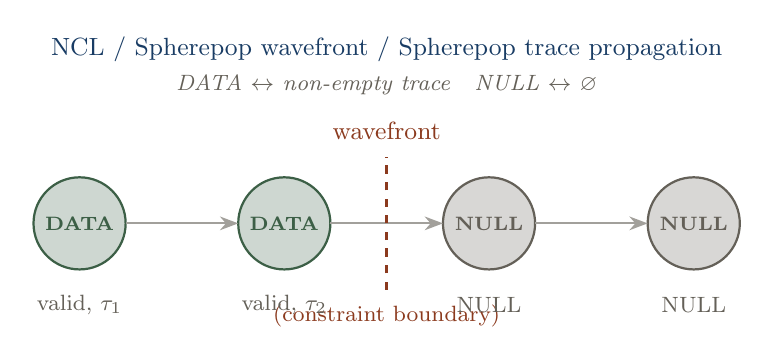
\begin{tikzpicture}[scale=1.3, >=Stealth]

  % --- nodes in a 4-stage pipeline (explicit to avoid \foreach colour issues) ---
  \fill[spsage!25] (0,0) circle (0.45);
  \draw[spsage, thick] (0,0) circle (0.45);
  \node[font=\scriptsize\bfseries, text=spsage] at (0,0) {DATA};

  \fill[spsage!25] (2,0) circle (0.45);
  \draw[spsage, thick] (2,0) circle (0.45);
  \node[font=\scriptsize\bfseries, text=spsage] at (2,0) {DATA};

  \fill[spgray!25] (4,0) circle (0.45);
  \draw[spgray, thick] (4,0) circle (0.45);
  \node[font=\scriptsize\bfseries, text=spgray] at (4,0) {NULL};

  \fill[spgray!25] (6,0) circle (0.45);
  \draw[spgray, thick] (6,0) circle (0.45);
  \node[font=\scriptsize\bfseries, text=spgray] at (6,0) {NULL};

  % --- gate connections ---
  \draw[->, thick, spgray!60] (0.45,0) -- (1.55,0);
  \draw[->, thick, spgray!60] (2.45,0) -- (3.55,0);
  \draw[->, thick, spgray!60] (4.45,0) -- (5.55,0);

  % --- wavefront boundary ---
  \draw[sprust, very thick, dashed]
    (3.0,-0.65) -- (3.0,0.65);
  \node[font=\small, text=sprust] at (3.0,0.9)
    {wavefront};
  \node[font=\footnotesize, text=sprust] at (3.0,-0.9)
    {(constraint boundary)};

  % --- labels below ---
  \node[font=\footnotesize, text=spgray] at (0,-0.8) {valid, $\tau_1$};
  \node[font=\footnotesize, text=spgray] at (2,-0.8) {valid, $\tau_2$};
  \node[font=\footnotesize, text=spgray] at (4,-0.8) {NULL};
  \node[font=\footnotesize, text=spgray] at (6,-0.8) {NULL};

  % --- top label ---
  \node[font=\small, text=spblue] at (3, 1.7)
    {NCL / Spherepop wavefront / Spherepop trace propagation};
  \node[font=\footnotesize\itshape, text=spgray] at (3,1.35)
    {DATA $\leftrightarrow$ non-empty trace\quad
     NULL $\leftrightarrow$ $\varnothing$};

\end{tikzpicture}
\caption{\textbf{Constraint wavefront (NCL / Spherepop correspondence).}
  Stages carrying valid data (non-empty trace) are shaded; stages awaiting
  completion remain NULL. The wavefront advances only when local completeness
  conditions are satisfied. This is the discrete analogue of the option-space
  contraction sequence $X_0 \supseteq X_1 \supseteq \cdots$.}
\label{fig:wavefront}
\end{figure}


This behaviour is structurally analogous to NULL Convention Logic (NCL), a
framework for asynchronous digital circuit synthesis. NCL introduces a
distinguished NULL value representing the absence of valid data; gates produce
output only when completeness conditions are satisfied, otherwise asserting
NULL. The NULL state is not merely the absence of computation but a logical
value encoding incompleteness.

The structural correspondence is precise. In NCL, the NULL state corresponds
to the empty trace in irreversible evaluation. Both represent the absence of a
complete and valid configuration. In both systems, the response to
incompatibility is not propagation but termination.

\section{Stratification Revisited}
\label{sec:para:priest}

Within Priest's framework, null collapse occupies a precise position. At the
level of \docens{}, contradictory formulas remain expressible. At the level of
\utens{}, their evaluation produces a trajectory terminating in failure. At the
level of \ens{}, no fact of validity is generated: the trace is empty.

Thus contradiction is not a truth-bearing object at the level of \ens{}, but
the absence of any stable outcome. Paraconsistency is therefore not an
additional feature imposed on the system, but a direct consequence of
irreversibility: once evaluation is understood as collapse, contradiction
ceases to be explosive and becomes terminal.

\section{Wavefronts, Traces, and Fields}
\label{sec:para:wavefront}

The correspondence with NCL extends beyond the identification of null states to
reveal a shared dynamical structure: the propagation of a constraint-satisfying
wavefront. In NCL, computation proceeds through the advance of a data wavefront
from an all-NULL state. Valid data values propagate through gates only when
local completeness conditions are satisfied. The wavefront is entirely internal
to the symbolic structure; no external temporal coordination is required.

In the Spherepop calculus, evaluation proceeds by successive contraction of the
option space, yielding $X_0 \supseteq X_1 \supseteq \cdots \supseteq X_n$.
This sequence may be interpreted as a propagating front of admissibility: the
set of surviving configurations advances through the expression as constraints
are imposed. The terminal trace corresponds to the stabilisation of this front.

In the RSVP framework, the scalar field $\RSVPfield(x,t)$ encodes the local
density of compatible configurations. Its evolution reflects the propagation of
constraint through the system, and stable regions correspond to trace-dominated
structures where the configuration space has largely collapsed.

All three descriptions share a common form. Each system evolves by enforcing
local constraints; global structure emerges as the fixed point of this process.
Sequential behaviour corresponds to constraint chains, parallel behaviour to
independent reductions, and the NULL state to regions where no compatible
configuration survives.

%=============================================================
% NEW CHAPTER: CONSTRAINT SYSTEMS
%=============================================================

%-------------------------------------------------------------
\chapter{A Category of Constraint Systems}
\label{ch:constr}
%-------------------------------------------------------------

The identifications developed in the preceding chapter suggest that
asynchronous circuits, irreversible evaluation, and field dynamics instantiate
a common abstract structure. We now formalise this structure as a category of
constraint systems, within which each of these domains arises as a concrete
realisation.

\section{Prerequisites}

This chapter assumes basic category theory at the level of Mac~Lane's \textit{Categories for the Working Mathematician}, Chapter~1: objects, morphisms, functors, and natural transformations. Readers unfamiliar with category theory should read Appendix~A first, which introduces the category $\mathbf{Hist}$ and the collapse functor $F$ in a more elementary style. The collapse and constraint-system framework from Chapters~3 and~4 is assumed throughout.

\section{Constraint Systems}
\label{sec:constr:defn}

\begin{definition}[Constraint System]
\label{def:constraint-system}
A \emph{constraint system} is a triple $\mathcal{C} = (X, \mathcal{R}, \Phi)$
where $X$ is a state space equipped with a partial order $\preceq$,
$\mathcal{R}$ is a family of local compatibility relations on $X$, and
$\Phi : X \to X$ is a monotone contraction operator satisfying
$\Phi(x) \preceq x$ for all $x \in X$.
\end{definition}

Iteration of $\Phi$ generates a descending chain
$x \succeq \Phi(x) \succeq \Phi^2(x) \succeq \cdots$
which stabilises at a fixed point. The operator $\Phi$ encodes the elimination
of incompatible configurations; the partial order records the direction of this
elimination.

A constraint system is \emph{irreversible} if and only if $\Phi$ admits no
right inverse: equivalently, if distinct states may be mapped to the same
fixed point, in which case the preimage information is irrecoverably lost.

\section{The Category Constr}
\label{sec:constr:category}

\begin{definition}
Let $\mathbf{Constr}$ be the category whose objects are constraint systems and
whose morphisms $F : (X, \mathcal{R}, \Phi) \to (Y, \mathcal{S}, \Psi)$ are
functions $F : X \to Y$ such that $F(\Phi(x)) = \Psi(F(x))$ for all
$x \in X$, and $F$ preserves compatibility relations in the sense that
$x \mathrel{\mathcal{R}} x'$ implies $F(x) \mathrel{\mathcal{S}} F(x')$.
\end{definition}

Morphisms commute with collapse: they carry trajectories to trajectories and
preserve the structure of constraint propagation. The following is immediate.

\begin{proposition}[Fixed Points Preserved]
\label{prop:fixed-preserved}
If $\Phi(x^*) = x^*$, then $F(x^*)$ is a fixed point of $\Psi$.
\end{proposition}

\begin{proof}
$\Psi(F(x^*)) = F(\Phi(x^*)) = F(x^*)$. \qed
\end{proof}

\section{Three Functorial Realisations}
\label{sec:constr:functors}

Spherepop evaluation, NULL Convention Logic, and RSVP field dynamics each
define objects of $\mathbf{Constr}$.

In the Spherepop calculus, the state space is $\Expr$ with refinement of
option spaces as the partial order. The operator $\Phi_{\mathrm{SP}}$ applies
one reduction step. The evaluation map $\evalf$ is the limit of iterated
$\Phi_{\mathrm{SP}}$, and fixed points are precisely the elements of $\NF$.

In NULL Convention Logic, the state space consists of all wire assignments
taking values in $\{0, 1, \mathrm{NULL}\}$. The operator
$\Phi_{\mathrm{NCL}}$ enforces completeness conditions across all gates. Fixed
points are stable data configurations; the NULL state is the least element
under the partial order.

In the RSVP framework, the state space consists of field configurations
$(\RSVPfield, \RSVPvec, S)$ over a spatial manifold. The operator
$\Phi_{\mathrm{RSVP}}$ advances the field dynamics by one step. Fixed points
are stable field configurations; regions of maximal entropy correspond to null
states.

\begin{definition}[Functorial Realisations]
There exist functors
\[
  F_{\mathrm{SP}} : \mathbf{Expr} \to \mathbf{Constr}, \quad
  F_{\mathrm{NCL}} : \mathbf{Circ} \to \mathbf{Constr}, \quad
  F_{\mathrm{RSVP}} : \mathbf{Field} \to \mathbf{Constr}
\]
assigning to each system its underlying constraint structure, carrying
expressions, circuits, and fields to the corresponding monotone contraction
systems.
\end{definition}

\section{Universality}
\label{sec:constr:universal}

\begin{theorem}[Universality of Constraint Propagation]
\label{thm:universality}
Every system admitting a local compatibility structure and a monotone
elimination operator embeds into $\mathbf{Constr}$.
\end{theorem}

\begin{proof}[Proof (Sketch)]
Given such a system, define $\Phi$ as the operator eliminating incompatible
states. Monotonicity follows from the definition of elimination. This yields an
object of $\mathbf{Constr}$, and the embedding is given by the identity on
states. \qed
\end{proof}

\section{Identity as Fixed Point}
\label{sec:constr:identity}

Within $\mathbf{Constr}$, identity is characterised by fixed points.

\begin{proposition}[Identity as Invariance]
Identity in a constraint system is equivalent to invariance under collapse:
$x$ is identical to itself if and only if $\Phi(x) = x$.
\end{proposition}

The notion of identity in Spherepop (the trace), the stable signal
configuration in NCL, and the equilibrium state in RSVP all coincide as fixed
points of their respective contraction operators, and therefore as objects in
$\mathbf{Constr}$. The category makes this coincidence precise.

%=============================================================
% NEW CHAPTER: VARIATIONAL PRINCIPLES
%=============================================================

%-------------------------------------------------------------
\chapter{Variational Principles and Cartesian Closure}
\label{ch:variational}
%-------------------------------------------------------------

\section{Prerequisites}

This chapter assumes Chapter~14 and a working familiarity with the concept of a functional (a real-valued function on a space of configurations). Readers with a background in variational calculus or optimisation theory will find the framework immediately familiar. The cartesian closed category material in Section~15.3 assumes knowledge of products and exponentials in a category; readers new to these ideas should consult Appendix~A. The connection to the Curry--Howard correspondence is implicit and is not developed formally here.

\section{Energy as Incompatibility}
\label{sec:var:energy}

The categorical formulation of constraint systems establishes that evolution
proceeds through monotone elimination. We now refine this structure by
introducing a variational principle. The central claim is that the collapse
operator is not merely monotone, but directed by a functional whose
minimisation encodes compatibility.

\begin{definition}[Constraint Functional]
\label{def:constraint-functional}
Let $(X, \mathcal{R}, \Phi)$ be a constraint system. A \emph{constraint
functional} is a map $\mathcal{E} : X \to \mathbb{R}_{\geq 0}$ such that
$\mathcal{E}(x)$ measures the degree of incompatibility in configuration $x$,
and $\mathcal{E}(x^*) = 0$ if and only if $x^*$ is a fixed point of $\Phi$.
\end{definition}

\begin{proposition}[Energy Decrease]
\label{prop:energy-decrease}
The collapse operator $\Phi$ is energy-decreasing:
$\mathcal{E}(\Phi(x)) \leq \mathcal{E}(x)$.
\end{proposition}

\begin{proof}
$\Phi$ eliminates incompatible components. The measure of incompatibility
cannot increase under elimination. \qed
\end{proof}

This allows the evolution of a constraint system to be interpreted as a
discrete descent along $\mathcal{E}$. In the Spherepop calculus, the
constraint functional measures unresolved constraints and incompatible
commitments; each reduction step reduces this measure. In RSVP, the functional
measures structural tension or entropy gradient; the field dynamics relax this
tension over time.

\section{Variational Formulation of Identity}
\label{sec:var:identity}

Within the variational framework, identity admits a refined characterisation.

\begin{proposition}[Identity as Minimal Energy]
\label{prop:identity-minimal}
Identity corresponds to global minima of the constraint functional. In
Spherepop, this is the normal-form trace; in NCL, it is a stable data
configuration; in RSVP, it is a coherent field structure.
\end{proposition}

Thus the general claim of the monograph---that identity is what survives
collapse---acquires a variational form: identity is the configuration of
minimal incompatibility reachable from the initial state under irreversible
descent.

%------------------------------------------------------------------
% FIG 2 — Energy Landscape / Entropic Descent (Chapter 15)
%------------------------------------------------------------------
\begin{figure}[htbp]
\centering
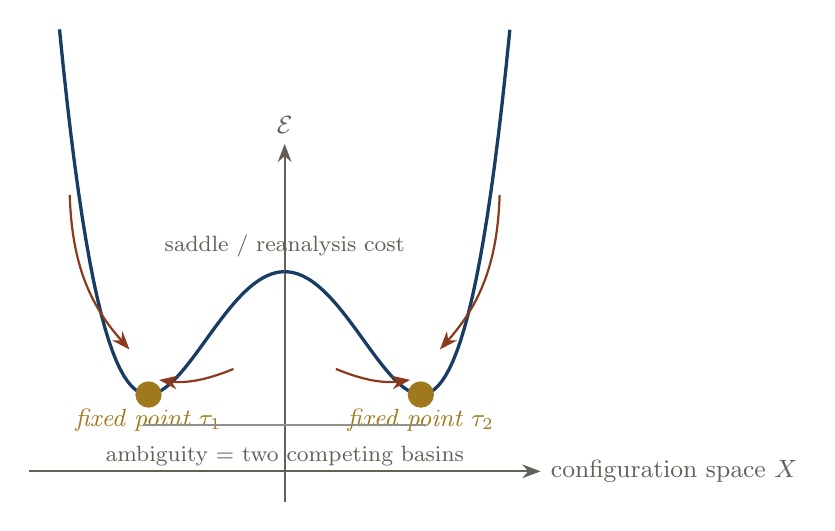
\begin{tikzpicture}[scale=1.3, >=Stealth]

  % --- axes ---
  \draw[->, thick, spgray] (-2.5,0) -- (2.5,0)
    node[right, font=\small] {configuration space $X$};
  \draw[->, thick, spgray] (0,-0.3) -- (0,3.2)
    node[above, font=\small] {$\mathcal{E}$};

  % --- double-well / collapse landscape ---
  \draw[spblue, very thick, domain=-2.2:2.2, samples=120]
    plot (\x, {0.38*\x*\x*\x*\x - 1.35*\x*\x + 1.95});

  % --- left local minimum (lx=-1.33, ly=0.75) ---
  \filldraw[spgold] (-1.33, 0.75) circle (3.5pt);
  \node[below, font=\small\itshape, text=spgold] at (-1.33, 0.70)
    {fixed point $\tau_1$};

  % --- right local minimum (rx=1.33, ry=0.75) ---
  \filldraw[spgold] (1.33, 0.75) circle (3.5pt);
  \node[below, font=\small\itshape, text=spgold] at (1.33, 0.70)
    {fixed point $\tau_2$};

  % --- descent arrows ---
  \draw[->, thick, sprust, shorten >=2pt]
    (-2.1, 2.7) to[bend right=20] (-1.48, 1.15);
  \draw[->, thick, sprust, shorten >=2pt]
    (-0.5, 1.0) to[bend left=15] (-1.28, 0.90);
  \draw[->, thick, sprust, shorten >=2pt]
    (2.1, 2.7) to[bend left=20] (1.48, 1.15);
  \draw[->, thick, sprust, shorten >=2pt]
    (0.5, 1.0) to[bend right=15] (1.28, 0.90);

  % --- saddle annotation ---
  \node[font=\footnotesize, text=spgray] at (0, 2.2)
    {saddle / reanalysis cost};
  \draw[spgray, dashed] (0,1.95) -- (0,2.1);

  % --- ambiguity annotation ---
  \draw[spgray!70, thick] (-1.38, 0.45) -- (1.38, 0.45);
  \node[below=4pt, font=\footnotesize, text=spgray] at (0, 0.45)
    {ambiguity = two competing basins};

\end{tikzpicture}
\caption{\textbf{Constraint functional $\mathcal{E}$ as incompatibility landscape.}
  Evaluation is entropic descent; fixed points are global or local minima.
  Two basins correspond to ambiguity; the saddle represents the cost of
  reanalysis (garden-path effect).}
\label{fig:energy}
\end{figure}


\section{Currying and Cartesian Closure via Constraint Propagation}
\label{sec:var:ccc}

The behavior of NULL Convention Logic and irreversible evaluation suggests that
higher-order structure may be realized without explicit functional abstraction.
The persistence of partially resolved states provides a direct realization of
currying.

In NCL, when a subset of inputs becomes valid while others remain NULL, the
circuit transitions to a partially resolved configuration. This intermediate
state is stable and encodes the effect of the supplied inputs on all future
behavior. It therefore plays the role of a function awaiting further arguments.

In the Spherepop calculus, fixing a partial input $a \in A$ restricts the
option space $X$ to a subspace $X_a$ of configurations compatible with $a$.
This residual system is stable under further evolution and represents all
admissible completions.

\begin{definition}[Residual System]
\label{def:residual}
Given a constraint system $(X, \Phi)$ and an input $a$, the \emph{residual
system} is the restricted system $(X_a, \Phi|_{X_a})$, where $X_a$ consists
of all configurations compatible with $a$.
\end{definition}

\begin{proposition}[Currying via Residualisation]
\label{prop:currying}
For each input $a$, the residual system $X_a$ determines a map on the
remaining input domain. This assignment defines a curried morphism
$\tilde{f}(a) = f(a, \cdot)$.
\end{proposition}

\begin{proof}
Fixing $a$ contracts $X$ to $X_a$, eliminating all configurations
incompatible with $a$. The remaining system evolves under further collapse,
yielding a unique output for each admissible remaining input. Thus $X_a$
defines a function on the residual domain. \qed
\end{proof}

Higher-order structure therefore emerges not from symbolic encoding but from
the geometry of constraint propagation. Currying is not added; it is forced by
irreversibility. Each committed input produces a definitive residual object
that serves as the partial application, because eliminated configurations
cannot be recovered.

\begin{theorem}[Cartesian Closure of Constraint Systems]
\label{thm:ccc}
Constraint systems admitting stable residual subspaces and deterministic
collapse form a cartesian closed category.
\end{theorem}

\begin{proof}[Proof (Sketch)]
Products are joint constraint spaces. Exponentials are residual systems
obtained through partial collapse. Evaluation is the continuation of collapse
within a conditioned space. The universal property of exponentials follows from
the correspondence between joint and sequential conditioning. \qed
\end{proof}

\section{Exponentials as Conditional Energy Landscapes}
\label{sec:var:exponentials}

Introducing the constraint functional $\mathcal{E}$ gives the cartesian closed
structure a variational interpretation.

\begin{definition}[Conditional Energy Object]
\label{def:conditional-energy}
Given a global functional $\mathcal{E} : A \times B \times C \to
\mathbb{R}_{\geq 0}$, the \emph{conditional energy object} determined by
$a \in A$ is the restricted functional $\mathcal{E}_a(b,c) = \mathcal{E}(a,b,c)$.
The exponential $B \Rightarrow C$ is the collection of such conditional
functionals indexed by $A$.
\end{definition}

\begin{proposition}[Currying as Conditioning]
\label{prop:currying-conditioning}
Currying corresponds to conditioning the global energy functional on a subset
of inputs: $\tilde{f}(a) = \arg\min_c \mathcal{E}_a(b,c)$ for each $b$.
\end{proposition}

\begin{theorem}[Conditional Variational Closure]
\label{thm:conditional-closure}
Constraint systems equipped with a compatible energy functional form a
cartesian closed structure in which exponentials correspond to conditional
energy landscapes and evaluation corresponds to conditional minimisation.
\end{theorem}

\begin{proof}[Proof (Sketch)]
Products are joint configuration spaces; conditioning induces residual systems
yielding exponentials; evaluation is minimisation within conditioned spaces.
The universal property follows from equivalence between joint and sequential
conditioning. \qed
\end{proof}

The consequence is that functions are not primitive objects but conditioned
energy landscapes: currying is the act of fixing variables and restricting the
system to a reduced domain; evaluation is descent to a minimum within that
domain. Logic, computation, and physical evolution are thus unified as
instances of the same principle: conditioning followed by minimisation under
irreversible descent.


%=============================================================
\part{Empirical Consequences and Conclusion}
%=============================================================

%-------------------------------------------------------------
\chapter{Empirical Signatures of Irreversible Structure}
\label{ch:empirical}
%-------------------------------------------------------------

The preceding chapters established a formal framework in which evaluation is
irreversible, identity is grounded in trace, and the distinction between
program, execution, and description collapses. These results were derived at
the level of abstract calculus. The present chapter considers their empirical
implications.

The aim is not to provide a complete experimental programme, but to identify
observable structures that would distinguish an irreversible model from one
based on reversible or lossless transformation. The central claim is that
irreversibility leaves characteristic signatures in the distribution,
stability, and interpretation of observable states.

\section{Prerequisites}

This chapter is the most speculative in the monograph and requires a broader background than the preceding chapters. Readers should be familiar with the collapse framework established in Part~II and the variational formulation of Chapter~15. Some acquaintance with dynamical systems, attractor theory, or the physics of entropy is helpful for the field-representation sections. The empirical predictions are stated as propositions rather than theorems; they are intended as research directions rather than established results. No experimental data is analysed.

\section{Asymmetry in Reconstruction}
\label{sec:empirical:asymmetry}

A direct consequence of the absence of a right inverse is that reconstruction
from observed outcomes is underdetermined. If an observable state corresponds
to a trace $\trace(E)$, then the set of possible antecedent structures is given
by the fiber $\preimgset{\trace(E)}$.

Empirically, this implies that systems governed by irreversible collapse will
exhibit reconstruction asymmetry. Forward evolution from an initial structure
will be well-defined and convergent, while inverse reconstruction from an
observed state will admit multiple incompatible hypotheses. This asymmetry may
be detected by comparing predictive and retrodictive performance. In a
reversible system the two are expected to align. In an irreversible system,
forward prediction remains stable while backward inference diverges across a
broad equivalence class.

\section{Entropy as Residual Constraint}
\label{sec:empirical:entropy}

The process of collapse may be interpreted as a progressive restriction of an
underlying option space. Let $X$ denote the set of admissible configurations
compatible with a given state. Each irreversible event reduces $X$ by
eliminating incompatible trajectories.

We may associate to $X$ a functional $\entropyF(X)$ measuring the residual
degrees of freedom consistent with the current trace. Under irreversible
evolution, this functional is non-increasing along trajectories of evaluation.
Empirically, this suggests that systems exhibiting irreversible collapse will
display monotonic contraction of accessible configuration space. Observable
states will appear increasingly constrained, even when no explicit conservation
law enforces such behaviour. Importantly, this contraction is not necessarily
accompanied by uniform dispersion. The reduction of $X$ may proceed through
highly structured eliminations, producing stable but non-uniform terminal
states.

\section{Field Representation and Trace Stability}
\label{sec:empirical:fields}

To model the spatial and temporal distribution of traces, we introduce a field
representation. Let $\RSVPfield(x,t)$ denote a scalar field encoding the local
density of compatible configurations at position $x$ and time $t$. Regions of
high density correspond to areas where multiple trajectories remain admissible,
while regions of low density indicate near-terminal collapse.

The evolution of this field reflects the propagation of constraint through the
system. Local reductions induce changes in $\RSVPfield$ that may extend beyond
their immediate domain, as eliminated configurations restrict neighbouring
possibilities. Empirically, this leads to the prediction of coherent regions in
which the field stabilises. These regions correspond to trace-dominated
structures, where the local configuration space has largely collapsed and the
system exhibits persistent behaviour.

\section{Persistence Without Reconstruction}
\label{sec:empirical:persistence}

A central feature of irreversible systems is that stable structures persist
without requiring the preservation of their generative history. The trace does
not encode the sequence of events that produced it, yet it remains robust under
further evolution. Empirically, this implies that systems may exhibit long-lived
structures whose origin cannot be uniquely reconstructed. Attempts to infer
their history will yield multiple incompatible explanations, all consistent with
the observed state.

Such persistence differs from stability in reversible systems, where invariants
are typically tied to conserved quantities or symmetries. In the present
framework, stability arises from the exhaustion of alternatives rather than the
preservation of structure.

\section{Ambiguity as Residual Branching}
\label{sec:empirical:ambiguity}

Not all trajectories collapse to a single trace. In some cases, the reduction
process terminates in a state that retains multiple compatible configurations,
corresponding to a non-singleton equivalence class at the level of the trace.
Empirically, such states manifest as ambiguity. The system supports multiple
interpretations that cannot be resolved without additional constraints. This is
not due to incomplete information, but to the persistence of branching within
the reduced configuration space.

\section{Irreversibility and Observational Limits}
\label{sec:empirical:limits}

The loss of preimage imposes intrinsic limits on observation. No measurement of
a trace can recover the full structure of its antecedent. Any attempt to do so
must rely on external assumptions or probabilistic reconstruction. This suggests
that certain forms of uncertainty are not epistemic but structural. They arise
not from a lack of information about an underlying reality, but from the fact
that the relevant information no longer exists within the system.

Empirical models that assume invertibility may therefore systematically
overestimate the recoverability of past states. Incorporating irreversibility
requires treating the preimage as fundamentally inaccessible.

\section{Synthesis}
\label{sec:empirical:synthesis}

The empirical consequences of irreversible collapse may be characterised as
follows. Systems governed by such dynamics exhibit asymmetry between prediction
and reconstruction, monotonic contraction of configuration space, persistence
of stable structures without recoverable histories, and the presence of
ambiguity as residual branching. These features do not depend on the specific
details of the reduction rules, but follow from the structural properties of
the evaluation map. The absence of a right inverse, the projection onto
equivalence classes, and the identification of identity with trace together
determine the observable behaviour.

%-------------------------------------------------------------
\chapter{Conclusion: Self-Reference Without Inverses}
\label{ch:conclusion}
%-------------------------------------------------------------

\textit{A system that has collapsed to its normal form no longer carries the
  history that produced it. What remains is not a record of the path, but the
  invariant that survived. Identity is this invariant.}

\medskip

The foregoing analysis has progressively removed a single, pervasive
assumption: that computation, logic, and meaning are fundamentally reversible.
Once this assumption is abandoned, the conceptual architecture of identity
undergoes a corresponding transformation. What remains is not a theory of
representation, but a theory of survival under collapse.

The Spherepop calculus provides a minimal formal setting in which this
transformation can be made explicit. By treating evaluation as an irreversible
contraction of possibility, it forces a distinction between what is constructed,
what is lost, and what persists. The central claim of this work is that identity
resides exclusively in the latter.

\section{Prerequisites}

The conclusion presupposes the entire preceding development. It is intended to be read after all other chapters, at which point no new definitions or theorems are introduced. Readers who have worked through the monograph in order will find this chapter acts as a compression of the argument rather than an extension of it.

\section{The Trace as Logica Ens}
\label{sec:concl:ens}

Through the stratification of \Cref{ch:priest}, the distinction between
\docens{}, \utens{}, and \ens{} becomes structurally grounded. The formal system
$(\Expr, \ruleR)$ constitutes the logic we teach: a theory of admissible
transformations. The reduction trajectories constitute the logic we use: a
practice of sequential commitment under constraint. The image
$\evalf(\Expr) \subseteq \NF$ constitutes logic itself: the set of invariant
traces that survive collapse.

In reversible systems these strata are implicitly conflated, because the
preimage of a result can in principle be reconstructed. In an irreversible
system, this conflation is no longer possible. The only stable object is the
trace $\trace(E)$. Accordingly, \ens{} is not a hidden semantic layer but the
terminal fixed point of reduction. Identity is not a property of an initial
configuration, but an invariant of a completed trajectory.

\section{The Redefinition of Self-Reference}
\label{sec:concl:quine}

The classical notion of a quine presupposes that syntactic structure can be
preserved or encoded across evaluation. This presupposition fails under
irreversible collapse (\Cref{prop:no-classical-quines}).

In Spherepop, a quine is redefined (\Cref{def:spherepop-quine}) as an
expression $Q$ satisfying $\evalf(Q) \tequiv Q$. The requirement is not
syntactic reproduction, but trace invariance. This eliminates the need for
representational duplication. A Spherepop quine does not reproduce its source;
it coincides with its result. The destruction of preimage is not an obstacle
but a condition of possibility. Self-reference is achieved precisely because
nothing remains except the invariant trace.

Thus, the quine becomes a limiting case of identity: an expression whose
evaluation yields no distinction between what it is, what it does, and what
it says.

\section{Language as Irreversible Computation}
\label{sec:concl:language}

The derivation of H-LFG (\Cref{ch:hlfg,ch:parse}) demonstrates that this
structure is not confined to abstract computation. An utterance is a sequence
of lexical events that irreversibly contracts a grammatical option space. The
c-structure records the historical organisation of these events as nested
scopes; the f-structure is the normal form of the resulting compatibility
network.

Grammaticality corresponds to the existence of a non-empty terminal trace;
ungrammaticality corresponds to total collapse (\Cref{prop:ungrammatical}).
Meaning is not an additional representational layer; it is the residual
structure that survives the elimination of incompatible trajectories. The
sentence does not encode its meaning; it is the trace of the process that made
it definite.

\section{The Irreducibility of the Trace}
\label{sec:concl:irreducibility}

The trace is not a derived or secondary object. It is not a summary of a prior
structure, nor a representation of an underlying process. It is the only object
that remains once the process of elimination has been completed.

Any attempt to treat the trace as an encoding of its preimage reintroduces the
assumption of reversibility. The absence of a right inverse shows that no such
encoding exists. The trace does not compress the preimage; it replaces it. There
is no deeper level at which the identity of the system may be recovered. The
trace is not the surface of a hidden structure. It is the terminal form of the
system itself.

\section{Identity as Terminal Trace}
\label{sec:concl:theorem}

\begin{theorem}[Identity as Trace]
\label{thm:identity-trace}
  Let $\evalf : \Expr \to \NF$ be an irreversible evaluation map with no right
  inverse. Then no expression has a recoverable preimage from its trace alone;
  the only stable notion of identity is the equivalence class $[E]_{\tequiv}$
  determined by the trace; and at normal-form fixed points, program, execution,
  and description coincide.
\end{theorem}

\begin{proof}
The first claim follows from \Cref{prop:no-right-inverse}. The second follows
from \Cref{def:identity} together with \Cref{lem:trace-adequacy}, which shows
that the coarsest observable criterion is the trace equivalence $\tequiv$.
The third follows from \Cref{thm:pec}. \qed
\end{proof}

\section{Temporal Finality}
\label{sec:concl:time}

Irreversibility introduces a fundamental directionality into the system.
Reduction proceeds from greater structural multiplicity to lesser structural
multiplicity, and this process cannot be reversed. This directionality is not
imposed externally but arises from the internal logic of collapse. Each step
reduces the available options, and no step restores them.

The trace marks the endpoint of this sequence. It is not a state that may be
revisited or revised, but a terminal condition. Temporal finality is not an
additional assumption, but a consequence of the structure of evaluation.

\section{Identity Without Origin}
\label{sec:concl:identity}

The relocation of identity from preimage to trace has a final implication.
Identity no longer depends on origin. Two expressions with distinct histories
may share the same identity if they collapse to the same trace. This does not
erase history, but it deprives history of its role as a criterion of identity.
The event word records the path taken, but identity is determined by what
survives.

Identity is forward-defined rather than backward-defined. It is not what
something was, but what it has become after the elimination of all incompatible
alternatives.

\section{Final Implication}
\label{sec:concl:final}

The consequence is not merely technical. It is ontological.

In a finite system, possibilities are progressively eliminated until only a
stable configuration remains. That configuration is not a snapshot of an
underlying essence; it is the residue of a history that can no longer be
undone. To ask what something is is therefore to ask what remains after all
incompatible alternatives have been excluded.

Self-reference without inverses is the only form of self-reference available
under these conditions. It does not consist in pointing back to an origin, but
in coinciding with the endpoint of a process.

Spherepop makes this visible in its simplest form. The bubbles of possibility
are transient; their popping is irreversible. What persists is the structure of
that collapse. And it is this structure---this trace---that constitutes
identity.

%------------------------------------------------------------------
% FIG 7 — Fixed-Point Identity / Quine Loop (Conclusion)
%------------------------------------------------------------------
\begin{figure}[htbp]
\centering
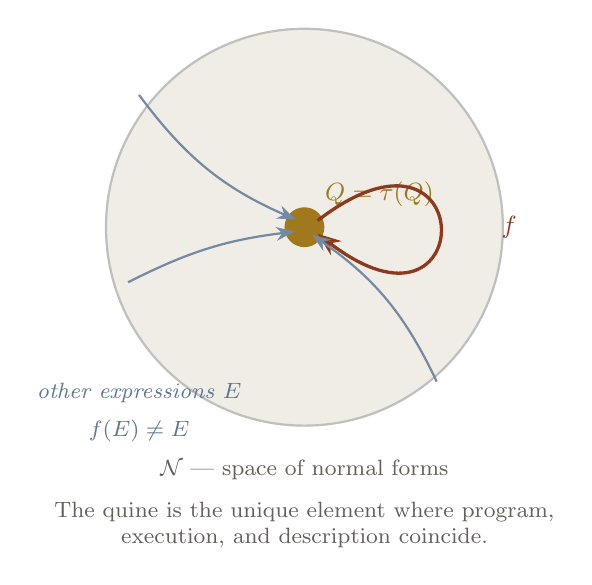
\begin{tikzpicture}[scale=1.4, >=Stealth]

  % --- background disc (the trace space) ---
  \fill[splightgray] (0,0) circle (1.8);
  \draw[spgray!40, thick] (0,0) circle (1.8);
  \node[font=\footnotesize, text=spgray] at (0,-2.2)
    {$\NF$ — space of normal forms};

  % --- fixed point (gold) ---
  \filldraw[spgold] (0,0) circle (5pt);
  \node[above right, font=\small\bfseries, text=spgold] at (0.1,0.1)
    {$Q = \trace(Q)$};

  % --- self-loop: collapse returns to same point ---
  \draw[->, very thick, sprust]
    (0.12,0.06)
    .. controls (1.6,1.2) and (1.6,-1.2) ..
    (0.12,-0.06);
  \node[right, font=\small\bfseries, text=sprust] at (1.7,0)
    {$\evalf$};

  % --- outer trajectories converging ---
  \draw[->, thick, spblue!60]
    (-1.5,1.2) to[bend right=15] (-0.08,0.07);
  \draw[->, thick, spblue!60]
    (1.2,-1.4) to[bend right=15] (0.07,-0.07);
  \draw[->, thick, spblue!60]
    (-1.6,-0.5) to[bend left=10] (-0.09,-0.04);

  % --- label for convergence ---
  \node[font=\footnotesize\itshape, text=spblue!70] at (-1.5,-1.5)
    {other expressions $E$};
  \node[font=\footnotesize\itshape, text=spblue!70] at (-1.5,-1.85)
    {$\evalf(E) \neq E$};

  % --- annotation ---
  \node[font=\footnotesize, text=spgray, align=center] at (0,-2.7)
    {The quine is the unique element where program,\\
     execution, and description coincide.};

\end{tikzpicture}
\caption{\textbf{Self-reference as fixed-point identity.}
  The Spherepop quine~$Q$ satisfies $\evalf(Q) \tequiv Q$: collapse
  returns $Q$ to itself. All other expressions are carried to distinct
  traces; only at the fixed point do program, execution, and description
  collapse into one object.}
\label{fig:quineloop}
\end{figure}

\medskip
\noindent
\textit{Identity is not preserved through evaluation; it is produced by
collapse.}

%=============================================================
%-------------------------------------------------------------
\chapter{Summary and Everyday Analogies}
\label{ch:summary}
%-------------------------------------------------------------

\section{Prerequisites}

This chapter assumes the full preceding monograph. It is intended to be read
after all other chapters. No new definitions or theorems are introduced.
The purpose is twofold: to provide a compressed restatement of the central
argument for readers who wish to survey the work before engaging it in detail,
and to offer a series of everyday analogies that make the formal claims
concrete without diluting them.

\section{The Central Argument in Brief}

This monograph has developed a formal theory of identity and self-reference
for irreversible computational systems, using the Spherepop calculus as its
central model. The guiding insight is that evaluation, when properly understood
as an irreversible collapse rather than a reversible transformation, forces a
fundamental revision of how identity, meaning, and self-reference are to be
conceived.

In standard computational frameworks, evaluation is treated as a transformation
that preserves informational recoverability. By contrast, the Spherepop calculus
formalises evaluation as a many-to-one map $\evalf : \Expr \to \NF$, where
distinct expressions collapse to the same normal form. This map admits no right
inverse. The loss of preimage is therefore not incidental but structural.
Reduction proceeds through irreversible operations---popping, binding, and
refusal---that eliminate syntactic structure and contract the space of
possibilities. What remains after evaluation is not a transformed version of
the original expression, but a residue: a trace.

This irreversibility necessitates a relocation of identity. Since preimages are
destroyed, identity cannot be grounded in initial syntax or generative history.
Instead, identity is defined by trace equivalence. Two expressions are identical
if and only if they collapse to the same normal form. The trace, as the invariant
of evaluation, is the sole bearer of identity. All prior structure is contingent
and expendable.

This shift induces a divergence in the classical tripartite distinction
articulated by Graham Priest. The logic we teach, the logic we use, and the
logic that is the case no longer coincide. Within the present framework, the
formal system $(\Expr, \ruleR)$ constitutes the \docens{}, the reduction
trajectories instantiated by irreversible evaluation constitute the \utens{},
and the image $\evalf(\Expr) \subseteq \NF$---the set of terminal traces---constitutes
the \ens{}. Under irreversibility, these strata separate. The theory describes
possible reductions, practice executes particular histories, and the facts of
identity are determined only at the level of the terminal trace.

Self-reference must therefore be reformulated. Classical quines rely on the
preservation or reconstruction of syntactic structure, implicitly assuming
reversibility. In an irreversible system, such reconstruction is impossible.
The Spherepop analogue replaces reproduction with coincidence. A quine is
defined as an expression $Q$ such that $\evalf(Q) \tequiv Q$, where
equivalence is taken at the level of trace. At such fixed points, the
distinctions between program, execution, and description collapse. The object
is not a generator of itself but the endpoint of its own evaluation.

This computational framework extends naturally to language. The derivation of
a Historical Lexical-Functional Grammar shows that linguistic structure can be
understood as the trace of an irreversible process. An utterance is a sequence
of lexical events that progressively contracts a grammatical option space.
Constituent structure records the historical nesting of commitments, while
functional structure is the surviving trace of compatible constraints.
Grammaticality is defined by the existence of a non-empty terminal trace;
ungrammaticality corresponds to total collapse, where no compatible
configuration survives; ambiguity arises when multiple traces remain viable
at the terminal stage.

These results admit a unifying abstraction. Spherepop, NULL Convention Logic,
and field-based constraint dynamics are all instances of systems governed by
monotone contraction operators on spaces of possibilities. Evaluation is a
descent process that eliminates incompatibility. Identity corresponds to a
minimal configuration under a variational principle, where energy is interpreted
as unresolved contradiction.

The sheaf-theoretic formulation provides a precise mathematical articulation.
Histories form a presheaf over the poset of partial traces, ordered by
refinement. Grammaticality corresponds to the existence of a global section---a
consistent gluing of local histories into a single trajectory. Ambiguity
corresponds to the existence of multiple global sections; ungrammaticality
corresponds to the failure of gluing, yielding an empty terminal trace. Meaning
is not an additional layer of representation but the existence and structure of
sections over the base space.

The cumulative result is a redefinition of identity for finite systems. Identity
is not preserved through evaluation; it is produced by collapse. The trace is
the terminal fact, and no deeper layer remains accessible once irreversibility
has taken place. Self-reference, under these conditions, is not the capacity to
reconstruct one's origin but the condition of coinciding with the endpoint of
one's own transformation.

\section{The Denouement Analogy}

The process of evaluation is structurally analogous to the denouement of a
narrative. A system begins in a state of multiplicity, supporting many possible
trajectories. As evaluation proceeds, incompatible possibilities are
irreversibly eliminated. The terminal trace is the state that remains once all
alternatives have been discharged.

This is not a loose resemblance. In classical narrative theory, the denouement
is the final unravelling of the plot---the state of the story after all
conflicts have been resolved and all alternative possibilities for the characters'
fates have been closed off. In the Spherepop calculus, the evaluation process
performs exactly this operation. Each reduction step commits to a specific
direction and eliminates branches that are no longer compatible with the
accumulated history of commitments.

The terminal trace is the structural equivalent of the denouement. It is the
configuration that remains only after the tension of the computation---the
unresolved or unevaluated nested bubbles---has been fully discharged. The
identity of the system is not found in its initial source or opening state,
but in the specific, irreversible configuration that survives to the end. Just
as the conclusion of a narrative resolves ambiguity by fixing a single history,
the trace represents the final configuration in which no further reinterpretation
is possible within the calculus.

The analogy also illuminates the sheaf-theoretic picture. A story with a
genuine ambiguity---one that the text sustains to the end without resolution---is
formally equivalent to a grammatical utterance with multiple surviving traces.
The story supports more than one global section over its narrative base. The
denouement, when it arrives, selects among these sections, or in rare cases
leaves them genuinely unresolved. A story whose plot contradicts itself
catastrophically---whose events become mutually incompatible before a coherent
ending can be reached---corresponds to an ungrammatical utterance: gluing fails,
the terminal trace is empty, and no final identity is produced.

\section{Adaptation as Premature Collapse}

The distinction between preimage and trace is vividly illustrated by the
adaptation of a written narrative into film. A literary text permits prolonged
indeterminacy in the attributes of its characters. The reader constructs an
implicit bundle of compatible interpretations and carries it forward through
the unfolding of the narrative. A character's precise appearance, voice, and
physical presence may remain undetermined---or deliberately indeterminate---across
hundreds of pages. This corresponds to a high-entropy preimage: many expressions,
many compatible trajectories, all collapsing eventually to the same narrative
identity.

A film enforces early collapse. The moment a character appears on screen, the
casting instantiates a specific physical and temporal realisation. A particular
actor's body, face, and voice select one trajectory from the space of
possibilities. The resulting representation is not a translation of the
original but its trace under a many-to-one projection. Formally, the adaptation
acts as an evaluation map from the space of textual possibilities to the space
of cinematic instantiations, and this map is many-to-one.

Once the film fixes these properties, the original indeterminacy is irrecoverable.
No viewer can reconstruct the full space of interpretations that existed in the
text from the film alone. This is the core claim of Chapter~4: the preimage is
destroyed; only the trace remains.

Techniques such as non-linear editing and flashbacks do not restore the lost
preimage. Rather, they reparameterise the order of collapse, presenting local
segments of the trajectory out of sequence while preserving the same global
resolution. A flashback does not reopen the possibilities; it re-stages the
commitments, in a different order, that were already made. Ambiguity is not
preserved by non-linear structure---it is resolved under a different temporal
ordering of constraints.

This demonstrates that identity in narrative, as in computation, is not
preserved across representation. It is produced by the irreversible elimination
of alternatives. The character in the film is not the same object as the
character in the book; the film character is the trace of the book character
under a specific collapse schedule.

\section{Cooking as Irreversible Constraint Resolution}

A simpler and equally precise analogy is the preparation of a dish from a
recipe. A recipe specifies a space of admissible ingredient combinations and
procedural sequences, most of which are intersubstitutable within limits. At
the outset, the cook operates in a high-dimensional option space: which tomatoes,
how ripe, how many, combined in what order with which other ingredients.

Each step of preparation applies an irreversible constraint. Chopping eliminates
the original integrity of the vegetable; it cannot be restored. Heat transforms
structure at the molecular level; the transformation is one-directional. Salt
dissolved into liquid cannot be unsalted. Each operation pops a bubble, in
Spherepop terms, and the structure it organised is gone.

The finished dish is the normal form of the recipe's option space under the
cook's specific sequence of reductions. Two cooks following the same recipe may
produce dishes that are functionally equivalent---they serve the same purpose,
carry the same nutritional content, and taste similar---yet differ in every
microscopic detail. These two dishes are co-identical in the sense of
Chapter~5: they share the same trace under the relevant equivalence relation,
even though their preimages (the specific sequences of preparation) differ.

Ungrammaticality in this domain is a dish that cannot be completed. If the
constraints imposed by a recipe become mutually incompatible---too much salt
renders further reduction pointless; a protein coagulates beyond the
temperature window in which a sauce can form---the option space collapses
to empty and no valid final configuration is reachable. The dish is
ungrammatical: the gluing fails.

The recipe itself is logica docens: the formal specification. The cook's
practice is logica utens: the particular sequence of reductions actually
performed. The finished dish is logica ens: the terminal fact, the trace that
constitutes the identity of the meal. The distinction between these three
levels, forced by irreversibility, maps directly onto Priest's stratification
in Chapter~6.

\section{Memory as Trace Without Preimage}

Human memory provides a particularly compelling analogy because it exhibits the
core asymmetry of collapse in a domain everyone has directly experienced.
Memory does not preserve a recording of an event; it preserves a trace. The
event, in its full original structure---the precise sensory detail, the
emotional context, the order of subsidiary perceptions---is not recoverable
from the memory. What is recoverable is an invariant that survived the
encoding process, which is itself irreversible.

This is why two people who attended the same event carry memories that differ
in structural detail while agreeing on the identity of what occurred. Both
memories are elements of the same preimage fiber: they collapse to the same
trace under the encoding relation. The trace is the shared normal form, and
it carries no information about which specific experiential trajectory produced
it.

The impossibility of recovering the exact experiential preimage from a memory
trace is not a limitation of brain architecture; it is the structural property
of any irreversible encoding. Memory is a collapse map, and its fibers are
large. The subjective sense that one's memory is ``of'' the original event,
rather than of its trace, is precisely the phenomenological equivalent of
mistaking a quotient for its preimage.

Distortion and false memory arise when the trace is treated as if it were a
right inverse of the original encoding---as if it determined, rather than
merely surviving from, the event. The absence of such an inverse is the
content of Proposition~4.1, and it applies to human memory as directly as it
applies to Spherepop reduction.

\section{Law and the Accumulation of Irreversible Commitment}

Legal systems provide a domain in which irreversibility is explicitly
formalised. A judgment, once entered, is not reversed by recourse to the
original facts; it is revised, if at all, only by a further irreversible act:
an appeal, a new verdict, a legislative change. Each legal decision is a
reduction step that eliminates a space of alternative resolutions and commits
the system to a specific configuration.

The common-law doctrine of precedent is the formal expression of the
append-only dynamics described in Chapter~3. A precedent adds an entry to
the legal ledger that cannot be removed; subsequent decisions must be
consistent with it or must explicitly distinguish themselves from it. The
option space of future judgments is constrained by the accumulated trace of
past decisions. This is constraint monotonicity in the sense of
Definition~10.3.

Legal ambiguity---cases that are genuinely underdetermined by statute and
precedent---corresponds to multiple surviving traces. The option space has not
been collapsed to a single configuration by the accumulated constraints, and
the system supports more than one valid global section. Judgment in such cases
is an act of selection among sections: the judge performs a disambiguation
that the law, taken alone, could not.

Ungrammaticality in law is the condition of a legal instrument so internally
contradictory that no consistent interpretation survives. Such instruments are
voided: the legal equivalent of the empty trace. No judgment can be entered
that satisfies all the constraints simultaneously; gluing fails.

The statute itself is logica docens. The practice of jurisprudence is logica
utens. The body of settled law---the accumulated trace of irreversible
decisions---is logica ens. The Priest stratification is not a philosophical
abstraction imposed on the legal system; it is the natural description of
how legal systems actually work.

\section{Musical Performance as Ordered Collapse}

A musical score specifies a space of admissible performances. Tempo markings,
dynamic indications, and articulation marks each impose constraints on the
option space of possible realisations, but they do not fully determine it.
The score is logica docens: a specification with many compatible models.

Each act of performance is an irreversible realisation. A breath, an attack, a
fingering, the exact moment of a crescendo---these are reductions that commit
the performance to a specific trajectory through the option space. Once a
phrase has been played, it cannot be unplayed; the acoustic trace is fixed.
The performance proceeds as an append-only history: a sequence of commitments
from which no retreat is possible.

Two performances of the same score are co-identical in the relevant sense if
they are functionally equivalent under the audience's perceptual evaluation
map. They are elements of the same fiber---different histories that produce
the same trace. What makes a performance ``the same piece'' is not that it
reproduces the score exactly (an impossibility, and not even desirable) but
that its trace is equivalent to the traces produced by other performances
within the same equivalence class.

Improvisation is the limiting case. In improvised music, there is no score to
constitute a logica docens; the performer operates directly at the level of
logica utens, with the accumulated sonic trace as the only constraint on
future choices. The piece, in such a setting, has no preimage: it is nothing
other than its own trace, generated in real time. This is the musical analogue
of the Spherepop quine: a system whose identity is its own evaluation, without
reference to any prior specification.

\section{Closing Statement}

These analogies are not illustrations added to make the theory accessible.
They are instances of the same formal structure in different domains. Narrative
denouement, cinematic adaptation, the preparation of a dish, the formation of
memory, the accumulation of legal precedent, and the realisation of musical
performance all exhibit irreversible contraction of an option space, trace-based
identity, and the three-level stratification that Priest names but irreversibility
forces. The theory is not abstract in the sense of being disconnected from
experience. It is abstract in the correct sense: it captures the structure
that these diverse phenomena share.

Identity, in all of these domains, is not preserved through evaluation. It is
produced by collapse. The trace is what remains after all incompatible
alternatives have been irreversibly excluded. There is no deeper layer.
History that has completed its contraction is identity.


\appendix
\renewcommand{\chaptername}{Appendix}
%=============================================================

%-------------------------------------------------------------
\chapter{A Categorical Formulation of Trace and Collapse}
\label{app:categorical}
%-------------------------------------------------------------

The Spherepop framework can be recast in categorical terms as a system of
histories modulo irreversible collapse. This formulation makes precise the
notion that identity is determined not by preimage structure, but by invariants
under evaluation.

\section{The Category of Histories}
\label{app:cat:hist}

\begin{definition}[Category $\mathbf{Hist}$]
  Let $\mathbf{Hist}$ be the category whose objects are Spherepop expressions
  $E \in \Expr$ and whose morphisms $h : E \to E'$ are reduction sequences from
  $E$ to $E'$. Composition is concatenation; identities are empty sequences.
\end{definition}

Because reduction is irreversible, $\mathbf{Hist}$ is not a groupoid: morphisms
are not, in general, invertible. This non-invertibility is not a defect but the
defining structural feature.

\section{The Collapse Functor}
\label{app:cat:functor}

Define a functor $F : \mathbf{Hist} \to \mathbf{NF}$, where $\mathbf{NF}$ is
the discrete category on the set of normal forms. The functor maps each
expression to its normal form $F(E) = \trace(E) = \evalf(E)$, and maps every
morphism (reduction sequence) to the identity on its codomain.

The functor $F$ forgets all path information except what survives in the
terminal trace. It is a quotient functor in the sense that it collapses the
internal structure of $\mathbf{Hist}$ onto a discrete base.

\section{Traces as Terminal Objects}
\label{app:cat:terminal}

For each trace $\tau \in \NF$, the object $\tau$ is the terminal object in
the full subcategory of $\mathbf{Hist}$ consisting of all expressions reachable
to $\tau$: there exists a unique morphism $h_E : E \to \tau$ for each $E$ with
$F(E) = \tau$.

\begin{proposition}[Trace Uniqueness]
\label{prop:terminal}
  For each $E \in \Expr$, the trace $\trace(E)$ is the terminal object in
  the full subcategory of $\mathbf{Hist}$ generated by $E$.
\end{proposition}

\begin{proof}
By confluence and termination (\Cref{asm:confluence}), every reduction sequence
from $E$ terminates at $\trace(E)$, and this terminal object is unique. Any two
sequences from $E$ therefore yield the same endpoint, so there is exactly one
object reachable as a terminal in that subcategory. \qed
\end{proof}

\section{Idempotence and Projection}
\label{app:cat:idempotent}

The evaluation operator induces an idempotent endofunctor on $\mathbf{Hist}$:
$F \circ F = F$. This reflects the fixed-point property $\evalf(\evalf(E)) =
\evalf(E)$ established in \Cref{def:fixedpoint}. Thus $F$ acts as a projection
from the category of histories onto the subcategory of traces.

\section{Identity as a Universal Property}
\label{app:cat:universal}

\begin{theorem}[Identity as Terminal Trace]
\label{thm:cat-identity}
  Two expressions $E, E' \in \Expr$ are co-identical (in the sense of
  \Cref{def:identity}) if and only if $F(E) = F(E')$, i.e., they are mapped
  to the same object by the collapse functor $F$.
\end{theorem}

\begin{proof}
By definition, $E \tequiv E'$ iff $\trace(E) = \trace(E')$ iff $F(E) = F(E')$
in $\mathbf{NF}$. \qed
\end{proof}

This formulation makes explicit that identity is a property of the image of
$F$, not of the internal structure of objects in $\mathbf{Hist}$.

\section{The Tripartite Correspondence as a Commuting Triangle}
\label{app:cat:triangle}

The tripartite correspondence of \Cref{thm:correspondence} can be elevated to
a commutative diagram. Let $\mathbf{Traj}$ be the category of reduction
trajectories, with $\eventword : \mathbf{Hist} \to \mathbf{Traj}$ recording
event words. Then:

\[
  \begin{tikzcd}
    \mathbf{Hist}
      \arrow[r, "\eventword"]
      \arrow[dr, "F"'] &
    \mathbf{Traj}
      \arrow[d, "\operatorname{NF}"] \\
    & \mathbf{NF}
  \end{tikzcd}
\]

\docens{} corresponds to the objects and morphisms of $\mathbf{Hist}$;
\utens{} to the trajectories in $\mathbf{Traj}$; and \ens{} to the discrete
category $\mathbf{NF}$.


%-------------------------------------------------------------
\chapter{Fibered Structure of Histories}
\label{app:fibered}
%-------------------------------------------------------------

\section{Prerequisites}

This appendix assumes Appendix~A and familiarity with the basic notions of
category theory introduced there. No prior knowledge of sheaf theory is
required; the construction is developed from the fibered picture and the
poset structure follows naturally. Readers with a background in algebraic
topology will recognise the Alexandrov topology as the standard construction
on a poset.

\section{Fibers as Spaces of Compatible Histories}

The collapse functor $F : \mathbf{Hist} \to \mathbf{NF}$ defines, for each
trace $\tau \in \NF$, the \emph{fiber category}
\[
  \mathbf{Hist}_\tau = F^{-1}(\tau),
\]
the full subcategory of all expressions and reduction sequences collapsing
to $\tau$. Distinct histories collapsing to the same trace are objects in the
same fiber. The collapse functor projects every object in a fiber to the same
base point and collapses every morphism to the identity there.

Ambiguity arises when a fiber contains multiple inequivalent objects that are
not connected by internal morphisms within $\mathbf{Hist}_\tau$. Two such
objects represent distinct derivational histories that share the same terminal
identity but cannot be transformed into one another without leaving the fiber.

\section{Sections as Consistent Interpretations}

A \emph{section} of $F$ is a functor $s : \mathbf{NF} \to \mathbf{Hist}$
satisfying $F \circ s = \mathrm{id}_{\mathbf{NF}}$. Since $\mathbf{NF}$ is
discrete, a section amounts to a choice function: for each trace $\tau$ it
selects one representative history $s(\tau) \in \mathbf{Hist}_\tau$ satisfying
$F(s(\tau)) = \tau$.

Different sections correspond to different canonical interpretations of the
same trace-level facts. In the linguistic setting, a section corresponds to a
particular parse selected from among all derivations compatible with the
terminal f-structure.

\begin{proposition}[Ambiguity as Multiplicity of Sections]
\label{prop:ambiguity-mult}
An utterance $u$ is ambiguous if and only if the fiber $\mathbf{Hist}_{\tau(u)}$
supports more than one inequivalent section.
\end{proposition}

\begin{proof}
Ambiguity means $|\FStr(u)| > 1$: multiple incompatible functional structures
survive collapse. Each surviving structure corresponds to a distinct choice
function on $\mathbf{Hist}_{\tau(u)}$, yielding a distinct section. The
sections are inequivalent because they select histories that collapse to
the same base but differ in their internal structure. \qed
\end{proof}

%-------------------------------------------------------------
\chapter{A Sheaf of Histories over the Space of Partial Traces}
\label{app:sheaf}
%-------------------------------------------------------------

\section{Prerequisites}

This appendix extends Appendix~B by equipping the space of traces with a
non-trivial topology. The construction converts the fibered picture into a
genuine sheaf, making locality and gluing mathematically precise rather
than metaphorical. Readers should be comfortable with the notion of a
presheaf (a contravariant functor into $\mathbf{Set}$ or $\mathbf{Cat}$)
and with the concept of a covering family in a site. The Alexandrov topology
on a poset is self-contained and explained below.

\section{The Poset of Partial Traces}

Extend $\NF$ to a partially ordered set $(\NF, \preceq)$ where
$\tau_1 \preceq \tau_2$ if and only if $\tau_1$ is a partial trace of
$\tau_2$: that is, $\tau_2$ refines $\tau_1$ by incorporating additional
irreversible commitments.

Intuitively, $\tau_1$ corresponds to an incompletely resolved structure---an
ambiguous or partially parsed state---while $\tau_2$ represents a more
definite collapse that has eliminated further alternatives. The refinement
relation is transitive (a partial trace of a partial trace is itself a
partial trace) and reflexive ($\tau \preceq \tau$), making $(\NF, \preceq)$
a genuine partial order.

\begin{definition}[Alexandrov Topology on $\NF$]
Equip $(\NF, \preceq)$ with the \emph{Alexandrov topology}: a subset
$U \subseteq \NF$ is open if and only if it is upward-closed,
\[
  \tau \in U \;\text{ and }\; \tau \preceq \tau' \;\Rightarrow\; \tau' \in U.
\]
\end{definition}

Open sets therefore correspond to collections of traces that are closed
under further refinement. If a partial trace belongs to an open set, every
more-determined trace also belongs. This reflects the fact that once a
trajectory has committed to a configuration, all more definite continuations
of that configuration remain in scope.

\section{The Presheaf of Histories}

\begin{definition}[Presheaf of Histories]
Define a presheaf
\[
  \mathcal{F} : \mathbf{NF}^{\mathrm{op}} \to \mathbf{Cat}
\]
by assigning to each trace $\tau$ its fiber category $\mathcal{F}(\tau) =
\mathbf{Hist}_\tau$. For a refinement $\tau_1 \preceq \tau_2$, define the
restriction functor
\[
  \rho_{\tau_2, \tau_1} : \mathbf{Hist}_{\tau_2} \to \mathbf{Hist}_{\tau_1}
\]
by truncating histories: a fully resolved trajectory in $\mathbf{Hist}_{\tau_2}$
is restricted to the prefix compatible with the coarser trace $\tau_1$.
\end{definition}

The restriction functors are required to satisfy the usual presheaf
coherence conditions: $\rho_{\tau,\tau} = \mathrm{id}$ and
$\rho_{\tau_3,\tau_1} = \rho_{\tau_2,\tau_1} \circ \rho_{\tau_3,\tau_2}$
for $\tau_1 \preceq \tau_2 \preceq \tau_3$.

\section{Local Compatibility and the Gluing Condition}

Let $\{\tau_i\}_{i \in I}$ be a family of partial traces whose least upper
bound exists in $(\NF, \preceq)$:
\[
  \tau = \bigvee_{i \in I} \tau_i.
\]
A family of histories $\{E_i \in \mathbf{Hist}_{\tau_i}\}_{i \in I}$ is
\emph{compatible} if the restrictions agree on all pairwise overlaps:
\[
  \rho_{\tau_i, \tau_{ij}}(E_i) = \rho_{\tau_j, \tau_{ij}}(E_j),
  \quad \text{where } \tau_{ij} = \tau_i \wedge \tau_j.
\]

\begin{theorem}[Sheaf of Histories]
\label{thm:sheaf}
The presheaf $\mathcal{F}$ satisfies the sheaf condition: for every compatible
family $\{E_i\}_{i \in I}$, there exists a unique global history
$E \in \mathbf{Hist}_\tau$ such that $\rho_{\tau, \tau_i}(E) = E_i$ for all
$i \in I$.
\end{theorem}

\begin{proof}[Proof (Sketch)]
The unique global history $E$ is constructed by assembling the compatible
partial trajectories into a single reduction sequence over $\tau$. Uniqueness
follows from the compatibility conditions: any two global extensions of the
same compatible family must agree on all local pieces, and since the local
pieces cover the full trace $\tau$, they determine $E$ completely. Existence
follows from the termination and confluence of $\ruleR$
(\Cref{asm:confluence}): any compatible family of partial trajectories that
share an upper bound extends to a complete reduction sequence terminating
at $\tau$. \qed
\end{proof}

\section{Failure of Gluing and Ungrammaticality}

When the sheaf condition fails, no global history can be assembled from locally
compatible pieces.

\begin{proposition}[Ungrammaticality as Obstruction]
\label{prop:sheaf-ungramm}
An utterance $u$ is ungrammatical if and only if there is no global section
of $\mathcal{F}$ over the putative trace of $u$, equivalently, if the gluing
of locally compatible partial histories yields $\varnothing$.
\end{proposition}

\begin{proof}
A global section assigns to $u$ a consistent history compatible with all
local constraints. Ungrammaticality means $\FStr(u) = \varnothing$
(\Cref{prop:ungrammatical}): no compatible functional structure exists.
This is equivalent to the failure of gluing: the local compatibility
conditions imposed by the lexical events cannot be satisfied simultaneously,
so no global section exists. \qed
\end{proof}

This recovers the result $X_{\mathrm{final}} = \varnothing$ of the main text,
now expressed as a topological obstruction: the local data cannot be extended
to a coherent global configuration over $\tau$.

\section{Ambiguity as Non-Unique Global Section}

\begin{theorem}[Ambiguity as Multiplicity of Global Sections]
\label{thm:ambiguity-section}
An utterance $u$ is ambiguous if and only if the sheaf $\mathcal{F}$ admits
more than one inequivalent global section over the trace of $u$.
\end{theorem}

\begin{proof}
Each global section assigns to $u$ a complete history $E$ satisfying all
local compatibility conditions. Ambiguity means that $|\FStr(u)| > 1$:
multiple incompatible functional structures each survive collapse
(\Cref{def:ambiguity}). Each surviving structure determines a distinct
global section, since distinct functional structures correspond to distinct
trajectories through the constraint space. These sections are inequivalent
because they select histories that differ as objects in $\mathbf{Hist}_\tau$.
\qed
\end{proof}

Each section represents a distinct interpretation compatible with the same
terminal trace: the same surface sequence of lexical events, the same
resulting f-structure identity, but a different path of derivational
commitment.

\section{Collapse as Sheaf Projection}

The evaluation map $E \mapsto \trace(E)$ can now be understood as the
projection from the sheaf $\mathcal{F}$ to its base space $\NF$. A chosen
global section $s : \NF \to \mathbf{Hist}$ selects a representative history
for each trace; the evaluation map then projects this history to its base
point, discarding all local structure above it.

Formally, the map
\[
  \evalf = \pi \circ s : \mathbf{NF} \to \mathbf{NF}
\]
is the identity (by definition of section). All higher-order structure---local
compatibility, branching histories, alternative sections---is discarded in
this projection.

\begin{proposition}[Quine as Degenerate Section]
\label{prop:quine-section}
A Spherepop quine $Q$ with $\evalf(Q) \tequiv Q$ corresponds to a degenerate
section: the history $Q$ is already fully determined by its trace, admitting
no further refinement and no alternative realisation.
\end{proposition}

\begin{proof}
The quine condition $\evalf(Q) \tequiv Q$ means that $Q$ and its trace lie
in the same equivalence class: the fiber $\mathbf{Hist}_{\trace(Q)}$ contains
$Q$ as its unique representative up to trace equivalence. The section over
$\trace(Q)$ has no choice: it must select $Q$. There is exactly one global
section through $Q$, and the sheaf at $\trace(Q)$ is a singleton. \qed
\end{proof}

\section{The Complete Sheaf-Theoretic Correspondence}

The sheaf formulation yields a precise dictionary between linguistic and
sheaf-theoretic notions. The base space $\NF$ carries identities as partial
and total traces. The fibers $\mathbf{Hist}_\tau$ carry histories realising
each identity. Global sections are coherent interpretations or parses. Gluing
is grammatical composition from locally compatible constraints. Failure of
gluing is ungrammaticality. Multiplicity of global sections is ambiguity.
The projection from the sheaf to its base is irreversible collapse.

Meaning is therefore not a point but a section over a space of partial traces.
Identity is the base point to which all sections project. Irreversibility
ensures that only the base point survives globally; all local variation is
confined to the sheaf structure above it.

%-------------------------------------------------------------
\chapter{Trace as Attractor: A Field-Theoretic Realisation in RSVP}
\label{app:rsvp}
%-------------------------------------------------------------

\section{Prerequisites}

This appendix assumes Appendices~A through~C, familiarity with partial
differential equations at the level of a first course in mathematical
physics, and basic acquaintance with the RSVP framework. The field equations
introduced here are presented heuristically; they are intended to
establish the structural correspondence between the sheaf of histories and
entropic field dynamics rather than to develop RSVP as a complete physical
theory. Readers without a physics background may read this appendix as
providing a continuous-space geometric intuition for the discrete algebraic
constructions of the preceding chapters.

\section{The RSVP Field as Semantic Substrate}

Let the RSVP system be defined over a smooth manifold $M$ equipped with
three fields: a scalar density $\RSVPfield(x,t)$, a vector flow
$\RSVPvec(x,t)$, and an entropy field $S(x,t)$. These fields evolve
according to coupled local equations expressing conservation, transport, and
dissipation.

We interpret the space of partial traces $(\NF, \preceq)$ as a discretisation
of regions in $M$. Each trace $\tau$ corresponds to a coherent field
configuration:
\[
  \tau \;\longleftrightarrow\; (\RSVPfield_\tau,\, \RSVPvec_\tau,\, S_\tau).
\]
Traces are therefore not merely symbolic objects but stable field patterns.
The refinement order $\preceq$ corresponds to the inclusion of spatial
regions in $M$: $\tau_1 \preceq \tau_2$ when the field configuration of
$\tau_2$ contains that of $\tau_1$ as a coherent subsystem.

\section{Histories as Trajectories in Field Configuration Space}

Each history $E \in \mathbf{Hist}$ corresponds to a trajectory through the
space of field configurations:
\[
  E : t \mapsto (\RSVPfield(x,t),\, \RSVPvec(x,t),\, S(x,t)).
\]
The reduction operations of the Spherepop calculus correspond to local
deformations of the field. The $\bind$ operator constrains compatible regions
of $\RSVPfield$, reducing entropy locally by eliminating configurations that
are incompatible with the imposed constraint. The $\pop$ operator eliminates
unstable configurations, collapsing regions of high curvature in the scalar
field toward nearby stable patterns. The $\refuse$ operator removes
incompatible trajectories, increasing the entropy gradient in regions
where no stable continuation exists.

The category $\mathbf{Hist}$ is therefore realised as a space of dynamical
flows over $M$: objects are field configurations (positions in configuration
space), and morphisms are trajectories (paths between configurations governed
by the field equations).

\section{Collapse as Entropic Descent}

The evaluation map $\evalf : \Expr \to \NF$ corresponds to the long-time
limit of field evolution. The scalar field evolves according to a
reaction-diffusion-advection equation of the form
\[
  \frac{\partial \RSVPfield}{\partial t}
  = D \nabla^2 \RSVPfield
    + \RSVPvec \cdot \nabla \RSVPfield
    + R(\RSVPfield - \RSVPfield^3),
\]
coupled with entropy dynamics satisfying the second law:
\[
  \frac{\partial S}{\partial t} \geq 0.
\]
The diffusion term $D \nabla^2 \RSVPfield$ smooths local irregularities.
The advection term $\RSVPvec \cdot \nabla \RSVPfield$ transports structure
along the flow field, implementing directed constraint propagation. The
reactive term $R(\RSVPfield - \RSVPfield^3)$ drives the field toward the
double-well potential minima, encoding the discrete commitments of reduction.

Under these dynamics, trajectories evolve toward low-entropy attractors. The
long-time limit
\[
  \lim_{t \to \infty} E(t) = \trace(E)
\]
is the normal-form trace of $E$: the stable field configuration that the
trajectory converges to once all incompatible alternatives have been
dissipated.

\section{Fibers as Basins of Attraction}

For each trace $\tau \in \NF$, the fiber category $\mathbf{Hist}_\tau$
corresponds geometrically to the basin of attraction of the field
configuration $(\RSVPfield_\tau, \RSVPvec_\tau, S_\tau)$:
\[
  \mathbf{Hist}_\tau \;\longleftrightarrow\;
  \bigl\{ E : \lim_{t \to \infty} E(t) = \tau \bigr\}.
\]
Different histories collapsing to the same trace are therefore trajectories
within the same basin, approaching the same attractor along different paths.
Ambiguity corresponds to the presence of multiple nearby attractors with
comparable energy levels (metastable basins). The system may converge to
either attractor depending on small perturbations in the initial conditions,
exactly as an ambiguous utterance may resolve to either interpretation
depending on contextual cues. Ungrammaticality corresponds to trajectories
that fail to converge to any stable attractor: the field disperses rather
than contracting, and no finite-energy terminal configuration is reached.

\section{Sheaf Structure as Local Field Coherence}

The sheaf structure of Appendix~C acquires a geometric interpretation in the
RSVP framework. A local section over a region $U \subseteq M$ corresponds
to a locally coherent field patch: a restriction of the global field
configuration to $U$ that satisfies the field equations with boundary
conditions consistent with the surrounding constraints.

Compatibility of local sections means that the field patches match smoothly
on their boundaries: $\RSVPfield$ and its derivatives agree on the overlapping
region, and there is no discontinuity in the flow field $\RSVPvec$ that would
prevent extension. Gluing corresponds to forming a globally stable field
configuration from locally compatible patches: a solution to the field
equations over all of $M$ that restricts to each local patch correctly.

Failure of gluing corresponds to a topological obstruction: locally compatible
field patches cannot be assembled into a global solution. This occurs when
the boundary conditions imposed by different local regions are mutually
incompatible, preventing any smooth extension. Linguistically, this is the
field-theoretic realisation of ungrammaticality as the failure of gluing in
the sheaf of histories.

\section{Trace as Minimal Entropy Configuration}

Each trace $\tau$ can be characterised as a local minimum of the effective
functional
\[
  \mathcal{F}[\RSVPfield]
  = \int_M \Bigl( \|\nabla \RSVPfield\|^2 + V(\RSVPfield) \Bigr)\, \mathrm{d}V,
\]
where $V(\RSVPfield) = \frac{1}{4}(\RSVPfield^2 - 1)^2$ is a double-well
potential encoding the two stable values of a discrete commitment. The
gradient term penalises spatial inhomogeneity, driving the field toward
uniform configurations, while the potential term penalises departures from
the committed values $\pm 1$.

In this language, collapse corresponds to the minimisation of $\mathcal{F}$
under the constraint that the entropy $S$ is non-decreasing. Identity
corresponds to a stable critical point of $\mathcal{F}$: a field configuration
that cannot be further deformed without increasing $\mathcal{F}$. Irreversibility
corresponds to the dissipative dynamics: trajectories descend monotonically
in $\mathcal{F}$ and cannot ascend without violating the entropy condition.

\section{The Spherepop Quine as a Fixed-Point Attractor}

A Spherepop quine $Q$ satisfying $\evalf(Q) \tequiv Q$ corresponds, in the
field picture, to a trajectory that is already located within its attractor
basin from the outset:
\[
  E_Q(t) = \tau_Q \quad \text{for all } t \geq 0.
\]
The field configuration of $Q$ is already a stable critical point of
$\mathcal{F}$: no dissipative evolution is required because the system is
already in its minimal-energy state. A quine is therefore not a loop in time
but a static point in configuration space---a field pattern that the dynamics
would produce as a terminal state, but which is already present as an initial
condition. It requires no further collapse because it is already the attractor.

\section{Identity as Entropic Endpoint}

\begin{theorem}[Identity as Entropic Attractor]
\label{thm:identity-attractor}
In an RSVP-realised Spherepop system, the identity of an expression $E$ is
the field attractor $\tau_E$ toward which its trajectory converges under
entropy-driven dynamics:
\[
  \mathrm{id}(E) = \lim_{t \to \infty} E(t) = \tau_E.
\]
\end{theorem}

\begin{proof}[Proof (Sketch)]
Irreversibility ensures that $\mathcal{F}$ is non-increasing along
trajectories ($\partial \mathcal{F}/\partial t \leq 0$). The dynamics
therefore admit no limit cycles or divergent trajectories: every trajectory
either converges to a stable critical point or dissipates entirely.
Stable critical points of $\mathcal{F}$ correspond bijectively to elements
of $\NF$ (the discrete committed values of the double-well potential).
All trajectories that do not terminate at such a critical point are
eliminated by the entropy condition. Hence the identity of $E$---its
terminal stable configuration---is determined uniquely by the attractor. \qed
\end{proof}

\section{The Unified Picture}

The RSVP realisation completes a sequence of identifications that spans the
entire monograph. At the symbolic level, Spherepop reduction is a sequence
of discrete collapse operations on expressions. At the categorical level,
these operations form morphisms in the category $\mathbf{Hist}$, which
projects onto the discrete base $\mathbf{NF}$ via the collapse functor.
At the sheaf-theoretic level, the fibers of this projection organise into
a presheaf over $(\NF, \preceq)$ satisfying the gluing condition, making
locality and coherence mathematically precise. At the field-theoretic level,
the fibers correspond to basins of attraction of the RSVP dynamics, and
the global sections of the sheaf correspond to globally stable field
configurations.

In each representation, the same structure appears under a different
description. Identity is the fixed point of an iterated contraction. The
trace is the attractor. The preimage is the basin. The sheaf section is the
consistent global configuration. Irreversibility is the entropy condition
that prevents trajectories from ascending.

\begin{corollary}[Structural Unity]
The logic of irreversible computation, the structure of natural language
under H-LFG, and the dynamics of RSVP fields are not merely analogous. They
are three representations of a single abstract object: a contractive dynamical
system over a space of configurations, governed by the condition that
entropy does not decrease, whose fixed points are identities.
\end{corollary}

\bibliographystyle{plainnat}
\begin{thebibliography}{99}

%%--- Logic and Philosophy ---

\bibitem{priest2006contradiction}
Priest, G.\ (2006).
\textit{In Contradiction: A Study of the Transconsistent}.
Oxford University Press, 2nd edition.

\bibitem{priest2006revising}
Priest, G.\ (2006).
Revising Logic.
In \textit{The Law of Non-Contradiction: New Philosophical Essays},
eds.\ Priest, G., Beall, J.\,C., and Armour-Garb, B.
Oxford University Press.

%%--- Asynchronous Logic and NULL Convention ---

\bibitem{fantbrandt1996}
Fant, K.\,M.\ and Brandt, S.\,A.\ (1996).
NULL Convention Logic: A Complete and Consistent Logic for Asynchronous
Digital Circuit Synthesis.
\textit{Proceedings of the International Conference on Application Specific
Systems, Architectures, and Processors}, IEEE.

\bibitem{fant2005}
Fant, K.\,M.\ (2005).
\textit{Logically Determined Design: Clockless System Design with NULL
Convention Logic}.
Wiley-Interscience.

%%--- Computation and Lambda Calculus ---

\bibitem{barendregt1984}
Barendregt, H.\,P.\ (1984).
\textit{The Lambda Calculus: Its Syntax and Semantics}.
North-Holland.

\bibitem{church1941}
Church, A.\ (1941).
\textit{The Calculi of Lambda-Conversion}.
Princeton University Press.

\bibitem{backus1978}
Backus, J.\ (1978).
Can Programming Be Liberated from the von Neumann Style?
\textit{Communications of the ACM}, 21(8):613--641.

\bibitem{plotkin1977}
Plotkin, G.\,D.\ (1977).
LCF Considered as a Programming Language.
\textit{Theoretical Computer Science}, 5(3):223--255.

\bibitem{winskel1993}
Winskel, G.\ (1993).
\textit{The Formal Semantics of Programming Languages}.
MIT Press.

%%--- Type Theory and Category Theory ---

\bibitem{lambek1986}
Lambek, J.\ and Scott, P.\,J.\ (1986).
\textit{Introduction to Higher-Order Categorical Logic}.
Cambridge University Press.

\bibitem{maclane1998}
Mac\,Lane, S.\ (1998).
\textit{Categories for the Working Mathematician}.
Springer, 2nd edition.

\bibitem{borceux1994}
Borceux, F.\ (1994).
\textit{Handbook of Categorical Algebra}, vols.\ 1--3.
Cambridge University Press.

\bibitem{abramsky1993}
Abramsky, S.\ and Jung, A.\ (1993).
Domain Theory.
In \textit{Handbook of Logic in Computer Science}, Vol.\ 3.
Oxford University Press.

%%--- Term Rewriting ---

\bibitem{terese2003}
Terese (2003).
\textit{Term Rewriting Systems}.
Cambridge University Press.

%%--- Linguistics ---

\bibitem{kaplan1982}
Kaplan, R.\ and Bresnan, J.\ (1982).
Lexical-Functional Grammar: A Formal System for Grammatical Representation.
In \textit{The Mental Representation of Grammatical Relations},
ed.\ Bresnan, J. MIT Press.

%%--- Physics and Information Theory ---

\bibitem{landauer1961}
Landauer, R.\ (1961).
Irreversibility and Heat Generation in the Computing Process.
\textit{IBM Journal of Research and Development}, 5(3):183--191.

\bibitem{bennett1973}
Bennett, C.\,H.\ (1973).
Logical Reversibility of Computation.
\textit{IBM Journal of Research and Development}, 17(6):525--532.

\bibitem{jaynes1957}
Jaynes, E.\,T.\ (1957).
Information Theory and Statistical Mechanics.
\textit{Physical Review}, 106(4):620--630.

%%--- Computability and Possible Worlds ---

\bibitem{turing1936}
Turing, A.\,M.\ (1936).
On Computable Numbers, with an Application to the Entscheidungsproblem.
\textit{Proceedings of the London Mathematical Society}, 42:230--265.

\bibitem{kripke1963}
Kripke, S.\,A.\ (1963).
Semantical Considerations on Modal Logic.
\textit{Acta Philosophica Fennica}, 16:83--94.

\bibitem{lambek1980}
Lambek, J.\ (1980).
From Lambda-Calculus to Cartesian Closed Categories.
In \textit{To H.\,B. Curry: Essays on Combinatory Logic, Lambda Calculus and
Formalism}, eds.\ Hindley, J.\,R.\ and Seldin, J.\,P.
Academic Press.

\end{thebibliography}

%=============================================================
\end{document}
%=============================================================
